\documentclass[11pt,letterpaper,oneside]{phstylee}

\usepackage[mathscr]{eucal}
\usepackage[table]{xcolor}
\usepackage{makeidx}
%\usepackage[ansinew]{inputenc}
%\usepackage[latin1]{inputenc}
\usepackage[final]{pdfpages}
\usepackage[utf8x]{inputenc}
\usepackage[spanish,es-noquoting]{babel}
\usepackage{array}
%\usepackage{epsfig}
%\usepackage{psfig}
%\usepackage{subfigure}
%\usepackage[dvips]{graphicx}
\usepackage{cite}
\usepackage{amsfonts}
\usepackage{amsmath}
\usepackage{amssymb}
\usepackage{amsxtra}
\usepackage{varioref}
\usepackage{multicol}
\usepackage{float}
\usepackage{rotate}
\usepackage{rotating}
\usepackage{color}
\usepackage{enumerate}
\usepackage{pmat}
%\usepackage{theorem}
%\usepackage[pdftex]{graphicx}
\usepackage{graphicx}
%\usepackage{hangcaption}
\usepackage{latexsym}
%\usepackage{stmaryrd}
% \usepackage{euler}
\usepackage{amsthm}
\usepackage{dsfont}
\usepackage{epstopdf}
%\epstopdfsetup{outdir=.}
\DeclareGraphicsExtensions{.pdf,.png,.jpg}
\usepackage{caption}
\usepackage{subcaption}
\usepackage{multirow}
\setcounter{secnumdepth}{5}
\usepackage{algorithm}
\usepackage{algpseudocode}
\usepackage{booktabs}
%\usepackage{fancybox}
%\usepackage{hyperref}
%\usepackage[pdftex,bookmarks,colorlinks]{hyperref} 
%\hypersetup{colorlinks,linkcolor=blue,urlcolor=blue}
%%%%%%%%%%%%%%%%%%%%%
%      DIRECTORIO DONDE BUSCA LAS FIGURAS

\graphicspath{{img/}}
\usepackage{pifont}
\usepackage{textcomp}
\usepackage{subcaption}
\usepackage{pgf}
\usepackage{tikz}
\usepackage{listings}
\usepackage{afterpage}
\usetikzlibrary{shapes,arrows,positioning,calc,shadows}

\addto\captionsspanish{%
\def\bibname{Referencias}%
\def\tablename{Tabla}%
\def\listtablename{ÍNDICE DE TABLAS}%
\def\listfigurename{ÍNDICE DE FIGURAS}
}

\renewcommand{\listfigurename}{ÍNDICE DE FIGURAS}
\renewcommand{\listtablename}{ÍNDICE DE TABLAS}

\newcommand{\comm}[1]{
\noindent\fbox{\parbox{\textwidth}{\begin{center} #1 \end{center}
}}\\}

\usepackage{mdframed}

\newcommand{\midtilde}{\raisebox{0.5ex}{\texttildelow}}

\usepackage{multirow}
\usepackage{etoolbox}
%\patchcmd{\thebibliography}{\section*{\refname}}{}{}{}

\definecolor{colora}{RGB}{102,190,14}
\definecolor{colorb}{RGB}{174,128,3}
\definecolor{colorc}{RGB}{204,51,51}
\definecolor{colord}{RGB}{174,3,128}
\definecolor{colore}{RGB}{120,14,190}
\definecolor{colorf}{RGB}{30,76,201}

\renewcommand\thesubsubsection{\Alph{subsubsection}}

\addtolength{\topmargin}{-30pt}

\usepackage[colorlinks=false,linkcolor=black,citecolor=black,hidelinks]{hyperref} %Para evitar recuadros de links.
\linespread{1.1}
\makeindex
\spanishdecimal{.}
\allowdisplaybreaks


%%%%% FIXME (set status=final to remove all comments before submitting) %%%%%

\usepackage[footnote, status=draft, nosilent, nomargin]{fixme}
\fxsetup{theme=color, mode=multiuser} 
\FXRegisterAuthor{gc}{agc}{\color{red}Gonzalo's comment}
\FXRegisterAuthor{jg}{ajg}{\color{brown}Jairo's comment}

\usepackage{soul}
\newcommand{\sgcnote}[1]{\gcnote{\color{gray}{\st{#1}}}}
\newcommand{\sjgnote}[1]{\jgnote{\color{gray}{\st{#1}}}}
%%%%%


%%%%%%%%%%%%%%%%%%%%%%%%%%%%%%%%%%%%%%%%%%%%%%%%%%%%%%%%%%%%
%%%%%%%%%%%%%%%%%%%%%%%%%%%%%%%%%%%%%%%%%%%%%%%%%%%%%%%%%%%%

\begin{document}

\tikzset{
block/.style = {draw, fill=white, rectangle, minimum height=3em, minimum width=3em},
tmp/.style  = {coordinate}, 
sum/.style= {draw, fill=white, circle, node distance=1cm},
input/.style = {coordinate},
output/.style= {coordinate},
pinstyle/.style = {pin edge={to-,thin,black}}
}

%%--------------------PORTADA--------------------------------

\setcounter{tocdepth}{2}


\pagestyle{empty}


\begin{center}

\large \textbf{UNIVERSIDAD TÉCNICA FEDERICO SANTA MARÍA}

\vspace{3mm}

\normalsize DEPARTAMENTO DE ELECTRÓNICA

\vspace{3mm}

\normalsize VALPARAÍSO-CHILE

\vspace{4mm}
		\begin{figure}[H]
			\centering
			
\includegraphics[width=5.85cm]{usmLogo_1.png}
		\end{figure}
\vspace{2mm}

\Large{\bf SISTEMA DE ADQUISICIÓN DE DATOS PARA DETECTORES DE MUONES}

\vspace{10mm}



\large \textbf{JAIRO ESTEBAN GONZÁLEZ CABEZAS}

\vspace{10mm}

\normalsize
MEMORIA DE TITULACIÓN PARA OPTAR AL TÍTULO DE INGENIERO CIVIL ELECTRÓNICO

\vspace{5mm}

PROFESOR GUÍA

%\vspace{2mm}

DR. GONZALO CARVAJAL
\vspace{5mm}

PROFESOR CO-REFERENTE

%\vspace{2mm}

DR. HAYK HAKOBYAN

\vspace{10mm}

Julio, 2021


\end{center}



\cleardoublepage

\vspace{50mm}

\begin{flushright}
  {\emph{\\}}
 \vspace{3mm}
  {\emph{\\}}


 
\end{flushright}
\vspace{170mm}
\begin{flushright}
{\emph{\\}}
\end{flushright}


\newpage
\thispagestyle{empty}
\cleardoublepage


%%--------------------AGRADECIMIENTOS----------------------

\pagestyle{fancyplain}
\pagenumbering{roman}
\cleardoublepage
\newpage


%\chapter*{Agradecimientos}
%%Agradecimientos

agradecer
%\afterpage{\thispagestyle{empty}\null\newpage}
%

%%--------------------RESUMEN----------------------

%\chapter*{Resumen}
%Los muones son partículas subatómicas originadas por la interacción y decaimiento de otras partículas elementales. Los muones se originan principalmente por radiación cósmica proveniente del espacio exterior y son capaces de penetrar en la atmósfera, incluso llegando a la corteza terrestre y atravesando la materia que encuentran a su paso. Medir la energía de un muón luego de su paso a través de la materia permite conocer la densidad de los materiales atravesados, por lo que la detección de muones es un área de estudio interesante para análisis de terrenos y estructuras.

El ``Sistema de adquisición de datos para detectores de muones'' nace como un requerimiento del CCTVal (Centro Científico Tecnológico de Valparaíso) en  el marco del proyecto ``sTGC Minería'', cuyo objetivo es realizar tomografías muónicas de terreno minero mediante detectores sTGC. Un detector emite señales eléctricas que representan la posición y la energía asociadas al paso de un muon, por lo que se requiere un sistema de adquisición que capture estas señales y las entregue a un posterior sistema de análisis para la caracterización del muon detectado.

En esta memoria de titulación se desarrolla un sistema de adquisición prototipo que cumple las funciones de muestrear señales digitales provenientes de un detector, discriminar la autenticidad de la detección mediante la lectura de una señal externa de disparo, y enviar la información capturada hacia un computador externo con el fin de almacenar y procesar los datos adquiridos. El sistema de adquisición debe ser capaz de muestrear 16 señales digitales cuyos tiempos de duración están en el orden de los nanosegundos, y debe diseñarse pensando en su replicación y escalamiento para facilitar la conexión de detectores adicionales. El trabajo de diseñar este sistema sienta un precedente importante para CCTVal, por lo que el proceso de desarrollo y los conocimientos adquiridos se documentan conjuntamente en esta memoria y en el repositorio de Git asociado.

\textbf{Palabras claves:} Detectores sTGC,  Muones, FPGA, Adquisición de Datos.
%
%\newpage
%\thispagestyle{empty}
%\cleardoublepage
%
%\chapter*{Abstract}
%%abstract

abstract

\textbf {Keywords:} words, words.
%
%\newpage
%\thispagestyle{empty}
%\cleardoublepage

%%--------------------ÍNDICE---------------------------------
\tableofcontents

\newpage
\thispagestyle{empty}


\listoffigures

\newpage
\thispagestyle{empty}
\cleardoublepage

\listoftables

\newpage
\thispagestyle{empty}
\cleardoublepage

%%-------------------CAPÍTULOS-------------------------------

\pagenumbering{arabic}

\chapter{Introducción}
\label{cap:introduccion}
En este documento se detalla el trabajo realizado en torno al diseño, implementación y validación \gcnote{\sout{entiendo que estaras haciendo el diseño, implementacion, y validacion, cierto}} de un prototipo de \gcnote{\sout{prototipo? Para acotarlo mas.}} sistema de adquisición de datos para detectores de muones. Este sistema fue diseñado en base a indicaciones y requerimientos específicos del Centro Científico Tecnológico de Valparaíso (CCTVal) para aplicaciones de detección de particulas y muongrafía de terrenos mineros \gcnote{\sout{Incluir una breve frase sobre el origen y contexto de uso para el desarrollo. Por ejemplo: ''El sistema de adquisicion fue diseñado en base a indicaciones y requerimientos especificos del CERN/CCTval para ser usado en aplicaciones de .....''}}. El sistema fue implementado en una matriz de puertas lógicas programable en campo, o FPGA (por su sigla en inglés, Field-programable gate array) \gcnote{\sout{Introducir el acronimo la primera vez que se usa}} utilizando SystemVerilog. \gcnote{\sout{borre la frase, pero no es necesario poner \emph{hardware} en cursivas. Vas a usar demasiados terminos en ingles, asi que quedaria raro el texto. Deja los terminos en fuente normal, y despues se ve cuales vale la pena destacar.}}

El presente capítulo relata el contexto, las principales motivaciones que originan este proyecto de titulación, el planteamiento del problema, sus alcances y las contribuciones asociadas. Al final del capítulo se incluye además la organización del documento y detalles de cada capítulo.

\section{Contexto}
\gcnote{Articula mejor el texto para que fluya mejor. Estas usando frases cortas separadas por puntos seguidos, que lo hacen ver como un telegrama. Cada vez que termines un texto, leelo en voz alta siguiendo las reglas gramaticales del colegio, y eso te dara una idea de donde poner las puntuaciones. Si se lee muy golpeado o interrumpido es indicacion de que hay demasiados puntos, si te quedas sin aire en algun frase es indicacion de que falta una coma o la frase esta muy larga, etc.}

	El planeta tierra es constantemente bombardeado por rayos cósmicos, los cuales provienen del espacio exterior y corresponden principalmente a partículas cargadas, como protones y núcleos atómicos. \gcnote{\sout{que es lo que se caracteriza por viajar a grandes velocidades? Esto gramaticalmente se llama un \emph{dangling modifier}. Estudia en que consiste y evitalos en el resto del documento y para el resto de tu vida. Tambien tiene que ver con el exceso de puntuacion.}} El origen de estos rayos es variado, y aunque la fuente de algunos de estos rayos es desconocida, la mayor parte de ellos proviene de tormentas solares, agujeros negros e incluso eventos astronómicos asociados al origen del universo. La velocidad alcanzada por estas partículas cósmicas es tan grande, que entran en la categoría de partículas de altas energías, alcanzando desde unos cuantos GeV (Giga Electron Volts) para partículas provenientes del sol, hasta más de 1000 TeV para rayos originados en centros galácticos y agujeros negros. \gcnote{\sout{Falta tambien un contexto de donde provienen o algo asi (no aparecen de la nada) y por que son relevantes, aunque sea algo intuitivo para el lector comun y corriente.}}
	
	El estudio de los rayos cósmicos permite conocer detalles sobre eventos astronómicos lejanos, pero también da la oportunidad de dilucidar características propias de la materia atravesada por estas partículas.
	
	Los rayos cósmicos inciden en el planeta tierra e interactúan con la atmósfera terrestre, produciendo la ionización del medio y decayendo en partículas secundarias. Estas últimas vuelven a interactuar con otras partículas, generando una efecto en cadena y produciendo así una lluvia de rayos subatómicos sobre la corteza terrestre. La figura \ref{img:cosmic-ray} corresponde a una representación artística de la lluvia de partículas originada por radiación cósmica.
	
	Cerca del 70\% de las partículas que logran llegar a la superficie del planeta corresponden a muones. \gcnote{dangling modifier}Estos poseen la misma carga que un electrón, pero con una masa cerca de 200 veces mayor. \gcnote{dangling modifier}Esta característica, sumada a su altísima velocidad \gcnote{cuanto?}, permite que los muones pasen a través de la materia. \gcnote{dangling modifier. El ultimo que marco. Corregir en todo el documento.}Incluso, son capaces de alcanzar zonas bajo tierra durante el transcurso de su vida media, correspondiente a aproximadamente $2\mu s$.
	
	Al atravesar materia, los muones son absorbidos o su energía se ve disminuida. Detectarlos y medir su energía permite entonces conocer propiedades de la materia que ha sido atravesada por estas partículas. Por ejemplo, es posible realizar un mapa de densidad de terreno a partir de los cruces de muones, proceso conocido como muongrafía o tomografía muónica \gcnote{seria bueno ir dando referencias de literatura para estos conceptos, en caso de que el lector quiera saber mas al respecto. Dar tambien un ejemplo de aplicaciones practicas (mineria, topografia, otros.). Esto es en forma breve, y despues en el resto del capitulo explicas mas detalles de las aplicaciones especificas. COnsidera la motivacion como un trailer motivacional para que el lector quiera seguir viendo la pelicula. Detectar muones es aburrido, las aplicaciones que tiene este tipo de tecnologia en entornos productivos es lo interesante desde el punto de vista de ingenieria.}.
	
	Para llevar a cabo mediciones y análisis de detección de muones se requieren detectores, interfaces de lectura, análisis computacional, y por supuesto, un sistema de adquisición de datos capaz de  transformar las características físicas de eventos detectados a datos computables y analizables para extracción e interpretación de la información.
	
	\begin{figure}[h]
		\centering
		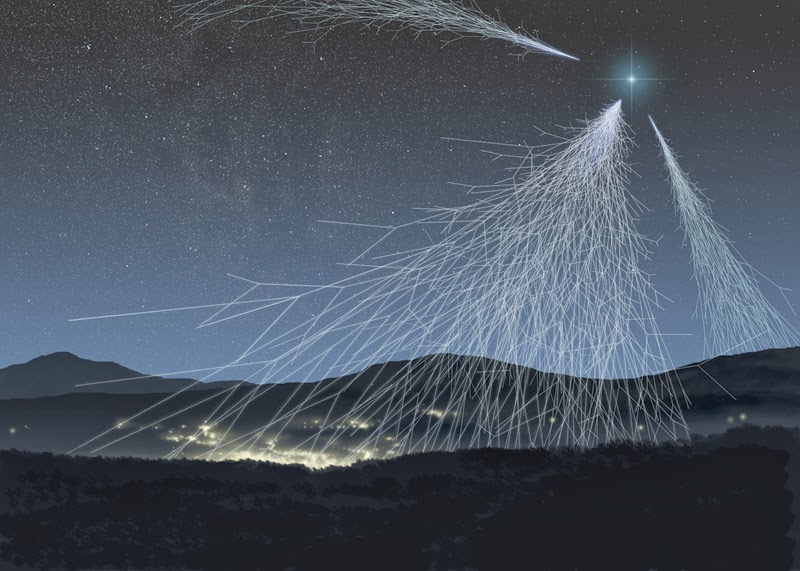
\includegraphics[scale=0.4]{cosmic_rays.jpg}
		\caption{Representación artística de rayos cósmicos y lluvia de partículas subatómicas sobre la corteza terrestre.}
		\label{img:cosmic-ray}
	\end{figure}
	
	
\section{Motivación}
	El ``Sistema de adquisición de datos para detectores de muones'' nace como un requerimiento del Centro Científico Tecnológico de Valparaíso (CCTVal) para aplicaciones de física de partículas, en el marco del proyecto ``sTGC Minería''. 
	
	Uno de los objetivos principales de ``sTGC Minería'' es realizar tomografías muónicas de terreno minero detectando partículas que provengan de radiación cósmica, método similar al que se utiliza para encontrar criptas y cavernas en pirámides egipcias\gcnote{interesante, pero da una referencia a algun articulo}. Estas tomografías sientan las bases para la detección de cavernas subterráneas y estimación de densidad en terrenos mineros. La figura \ref{img:muongrafia} corresponde a una muongrafía de un corte trasversal de terreno. \gcnote{explicar un poco mejor la figura. Que informacion util entrega esa figura? Que significa el mapa de colores?}

	
	Producto de la colaboración existente entre CCTVal y el experimento ATLAS, en CERN, el centro cuenta con las herramientas y conocimientos necesarios para la fabricación de detectores de muones en Chile. Los detectores de partículas a utilizar en ``sTGC Minería'' corresponden precisamente a unos basados en los detectores del espectrómetro de muones presente en el experimento ATLAS.
	
	\begin{figure}[h]
		\centering
		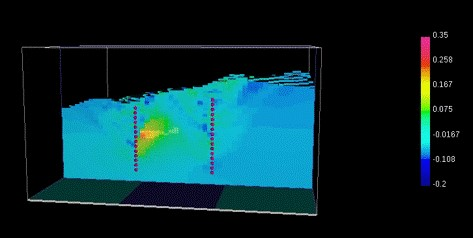
\includegraphics[scale=1]{Stgcgif.jpg}
		\caption{Imagen referencial de un mapa de calor para representación de densidades en un corte transversal de terreno.}
		\label{img:muongrafia}
	\end{figure}
	

\section{Planteamiento del Problema}
\label{sec:planteamiento}
	La detección de muones implica una serie de etapas y detectores desarrollados con tecnologías que se utilizan en experimentos tales como ATLAS, en CERN \gcnote{Introducir los acronimos}. Particularmente en ``sTGC Minería'', se requiere un sistema que sea capaz de captar las señales generadas por los detectores y que determine de manera fiable y precisa \gcnote{a que te refieres con fiable y precisa?} aquellas zonas del detector por las cuales ha pasado un muon.
	
	El ``Sistema de adquisición de datos para detectores de muones'' cumplirá con las funciones de adquirir, discriminar y estructurar la información captada desde el detector, para así contribuir a la tomografía muónica del terreno.
	
 	Como objetivo principal se tiene el detectar la posición del paso de muones en un detector de configuración matricial, indicando el o los cuadrantes \gcnote{no se han explicado lo de los cuadrantes ni cosa asociadas. Quizas debas mover las especificaciones tecnicas generales antes.} que han sido excitados por el paso de las partículas, de manera fiable y eficiente \gcnote{antes dijiste eficiente y precisa. Se consistente con el lenguaje tecnico, no es un reporte literario ni de poesia (lo cual no quiere decir que puede estar mal escrito).}, logrando captar gran \gcnote{cuantas? Evita el uso/abuso de terminos no cuantificables y subjetivos. Da al menos ordenes (decenas, cientos, miles?)}{cantidad de señales íntegramente \gcnote{que es integramente? que no sean corruptas o eticamente correctas?}.
 	
 	La figura \ref{img:sistema} ilustra el sistema de muongrafía de terreno considerando un solo detector de muones. Para su operación, utiliza dos detectores centelleantes secundarios, un sistema de coincidencias y una interfaz de lectura. El sistema de adquisición de datos capta y discrimina los pulsos generados según se correspondan con la señal de coincidencia asociada a los detectores centelleantes. La información resultante es comunicada a etapas posteriores para análisis de datos. \gcnote{Esto deberia ir antes. Ver comentarios anteriores.}
	
	Es requisito del proyecto que este sistema sea concebido como una herramienta adaptada para operar con detectores de mayor tamaño o con arreglos de detectores individuales, permitiendo el análisis de zonas de mayor área o el estudio de trayectorias de partículas con detectores superpuestos. Esto implica que el sistema debe ser de naturaleza modular y expansible, sobre todo en torno a la cantidad de señales que es capaz de procesar.  \gcnote{No queda claro que es lo que ya esta hecho y que es lo que haras tu? Estas haciendo el detector completo, o solo el sistema de adquisicion? Explicar mejor. Tambien dejar claro que es un prototipo de cierto tamaño.}
	
	Como objetivo secundario, el proyecto debe ser una herramienta replicable que esté disponible para ser utilizada en nuevos proyectos y experimentos del centro de investigación. Así mismo, el desarrollo y la documentación del proceso debe ser un aporte al conocimiento sobre la implementación de sistemas electrónicos para la detección y análisis de partículas utilizando estas tecnologías, ya que es uno de los primeros en ser desarrollados y probados por el centro. \gcnote{Esto ultimo deberia plantearse como una motivacion. ''Actualmente no se tiene conocimiento sobre esto, por lo que en este proyecto se busca adquirir experiencia practica...''}
	
	\begin{figure}[h]
		\centering
		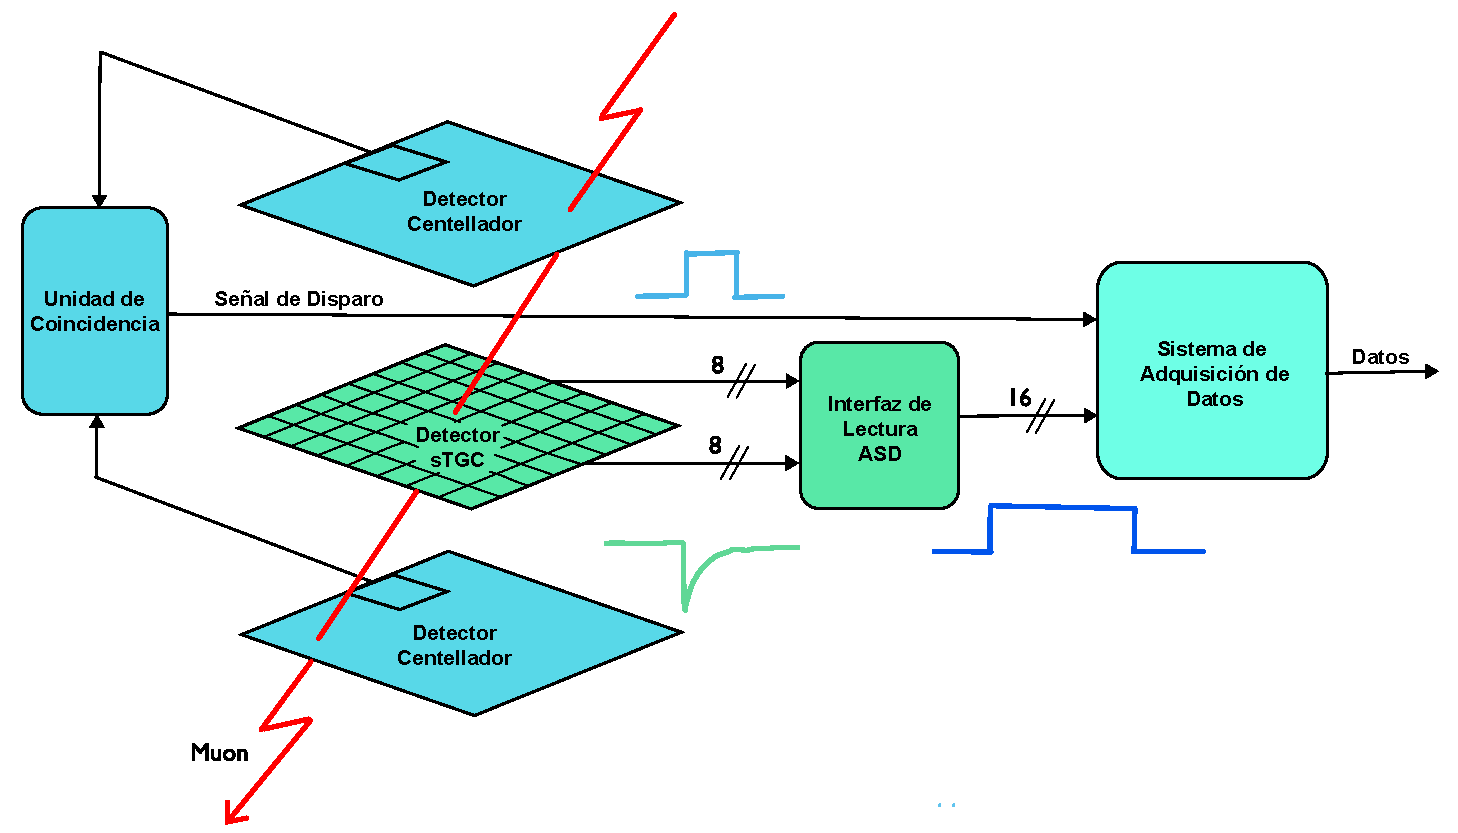
\includegraphics[scale=0.55]{sistema.pdf}
		\caption{Diagrama del sistema de muongrafía de terreno para un solo detector. Se incluyen en azul las formas de señal asociadas a la señal de disparo, eventos de detección, y lectura de pulsos.}
		\label{img:sistema}
	\end{figure}						

\section{Alcances y contribuciones}

\gcnote{Toda esta seccion debe ser mas concreta y especifica.}
	Se espera que este sistema sea capaz de generar información suficiente para representar la ubicación del paso de las partículas en la superficie del detector, determinando cuadrantes de $1cm^2$ que hayan sido excitados por el cruce de partículas.
	
	El sistema deberá ser capaz de captar cantidades pares arbitrarias de canales, discriminando partículas mediante la utilización de las señales de disparo disponibles.
	
	La información generada pasará a etapas siguientes de análisis detallado o de representación gráfica, por lo cual es importante que el sistema sea capaz de entregar información pertinentemente ordenada, procesada y seleccionada para dichos fines.
	
	Finalmente, uno de los principales aportes recae en la documentación respecto a entorno, operación y desarrollo del sistema en cuestión. Esto con el fin de facilitar la implementación del diseño en nuevos sistemas, permitir profundizar y mejorar la propuesta diseñada y entregar las herramientas al centro y a futuros estudiantes para operar dispositivos que posean etapas equivalentes.


\section{Organización del documento.}

	Este documento se estructura de la siguiente manera: \gcnote{demasiados capitulos. No deberian ser mas de 5 o 6.}
	
	\begin{itemize}
		\item El \textbf{Capítulo \ref{cap:art}} incluye el estado del arte en cuanto a dispositivos de adquisición de datos para partículas de altas energías.
		\item El \textbf{Capítulo \ref{cap:arq}} detalla la arquitectura propuesta para la realización de este proyecto, contemplando componentes y estructura del mismo.
		\item El \textbf{Capítulo \ref{cap:stgc}} describe las características del detector de partículas utilizado.
		\item El \textbf{Capítulo \ref{cap:asd}} resume las especificaciones del sistema de lectura para señales provenientes del detector, además de explicar su estructura y funcionamiento.
		\item El \textbf{Capítulo \ref{cap:sampling}} detalla la primera etapa de diseño de hardware, encargada de tomar muestras de los pulsos digitales provenientes de la etapa inmediatamente anterior.
		\item El \textbf{Capitulo \ref{cap:discriminator}} trata sobre el diseño para la etapa de discriminación del sistema de adquisición, la cual selecciona aquellos eventos temporalmente coincidentes con una señal de disparo.
		\item El \textbf{Capítulo \ref{cap:structure}} describe la etapa de estructuración de eventos y su diseño, en donde la información de pulsos capturados es asociada los canales y cuadrantes correspondientes.
		\item El \textbf{Capítulo \ref{cap:analysis}} detalla la etapa de análisis de datos para determinación del paso de partículas cargadas por el detector.
		\item El \textbf{Capítulo \ref{cap:sync}} trata sobre la etapa de sincronización y su diseño, en donde se coordinan eventos capturados por distintos detectores simultáneamente.
		\item El \textbf{Capítulo \ref{cap:comm}} se refiere a la etapa de comunicación serial, a través de la cual el sistema se comunica con computadores externos para envío de datos.
		\item El \textbf{Capítulo \ref{cap:test}} incluye pruebas realizadas en el sistema con el fin de comprobar funcionamiento y resultados del dispositivo.
		\item El \textbf{Capítulo \ref{cap:insights}} resume los resultados de experimentación y desempeño del sistema diseñado.
		\item El \textbf{Capítulo \ref{cap:conclusiones}} incluye las conclusiones finales y trabajo futuro propuesto a partir de lo realizado en este proyecto de titulación.
	\end{itemize}



\newpage
\thispagestyle{empty}
\cleardoublepage

%\chapter{Marco teórico}
%\label{cap:marco}
%\input{tex/MarcoTeorico.tex}
%
%\newpage
%\thispagestyle{empty}
%\cleardoublepage

\chapter{Estado del arte}
\label{cap:art}
%Estado del arte y arquitectura propuesta
Previo al diseño del sistema de adquisición de datos para detectores de muones, es pertinente conocer el estado del arte de otros sistemas de adquisición para física de partículas, con el fin de contrastar y rescatar las diferentes estrategias y tecnologías empleadas en la actualidad.

Como referencia para el diseño del sistema de adquisición, se han investigado detectores como los descritos en \cite{Basiladze2017Methods1} y \cite{Basiladze2017Methods2}, enfocados a detección de partículas en diferentes rubros y condiciones. En este capítulo se describen tres sistemas relacionados a esta temática, destacando ideas sobre el esquema general de adquisición de datos, tecnologías que se utilizan actualmente para construirlos y métodos para adquirir y procesar las señales captadas.

\section{LabPet II}
\label{par:labpet}
	Uno de los detectores estudiados es LabPet II \cite{Njejimana2013DesignImaging}, detector que posee un DAQ (Data Acquisition system) distribuido en tres etapas donde cada una de ellas está compuesta por una FPGA, tal como se ilustra en la Figura \ref{fig:njejimana}. Una primera etapa llamada \textit{Front-End board} se encarga de registrar tiempo, energía y posición de las partículas captadas; una segunda etapa llamada \textit{Hub board} ordena cronológicamente los eventos capturados, mientras que una tercera etapa llamada \textit{Coincidence board} agrupa detecciones coincidentes, calculando además la tasa de eventos aleatorios ocurridos. Esta última etapa es capaz de recibir datos desde múltiples Hub boards para luego enviarlos a un computador.
	
	%La Figura \ref{fig:njejimana} ilustra LabPet II \gcnote{dangling modifier. Estas cometiendo los mismos errores que antes.}. Se \gcnote{otro mas} compone de 3 FPGAs: una encargada de capturar las señales provenientes de los detectores, llamada \textit{Front-End board}; otra dedicada a ordenar los eventos y corregir datos, llamada \textit{Hub board}; y una última FPGA encargada de seleccionar eventos válidos y coincidentes, llamada \textit{Coincidence board}, la cual puede conectarse a múltiples Hub boards. \gcnote{Suena redundante con el parrafo anterior. Juntar y uniformar ambos parrafos.} Los resultados son enviados a un computador, el cual también permite configurar y ajustar parámetros en las Hub y Coincidence boards.
	
	Si bien los detectores de LabPet II están diseñados para otro tipo de partículas (positrones), la naturaleza de las señales es muy similar a los muones, y por lo tanto la lógica para su adquisición y procesamiento es comparable. Aún así, la cantidad de señales que es capaz de manejar dicho dispositivo ronda las 64 señales por módulo, a tasas cercanas a los 2 millones de eventos por segundo, las que comparativamente sobrepasarían las necesidades del sistema a desarrollar en este proyecto de titulación. Por ejemplo, los rayos cósmicos cruzan el planeta tierra a aproximadamente 1 rayo cósmico por minuto en un área de 1 cm$^2$ \sgcnote{cm y otras unidades no deberian ir en italicas. Italicas es para varibles en expresiones matematicas. Corregir en todo el documento.}, muy por debajo de lo que se espera en LabPET II. Replicar un sistema como LabPet II para sTGC minería sería factible, pero implicaría un uso de recursos mayor al realmente necesario \sgcnote{poco optimo? puede ser mas optimo? y mas mejor o menos mejor?}, ya que se podrían alcanzar los objetivos propuestos para sTGC minería con un sistema de menor tamaño, por ejemplo utilizando solo una FPGA por módulo de detección en vez de dos o tres.
	
	Del sistema de adquisición para LabPet II se destaca la utilización de multiplexores, serializadores/deserializadores y memorias de almacenamiento temporal (\textit{buffer}). Dada la naturaleza y cantidad de eventos, se hace necesario serializar la información, ya que de otro modo sería necesario construir dispositivos con múltiples puertos de entrada o incluir varios del mismo tipo. Además, debido a la frecuencia de los eventos, se hace obligatoria la existencia de \textit{buffers} para el almacenamiento de la información, permitiendo procesarlos y transmitirlos hacia etapas posteriores a tasas menores. Es destacable también la utilización de métodos para ordenar cronológicamente los eventos y la implementación del método TOT (Time-over-threshold)\cite{Orita2018TheSystem} para el cálculo de energía y datos temporales de pulsos analógicos. Este último es el método utilizado por la interfaz de lectura presente en el proyecto sTGC Minería.
	
	\begin{figure}[h]
		\centering
		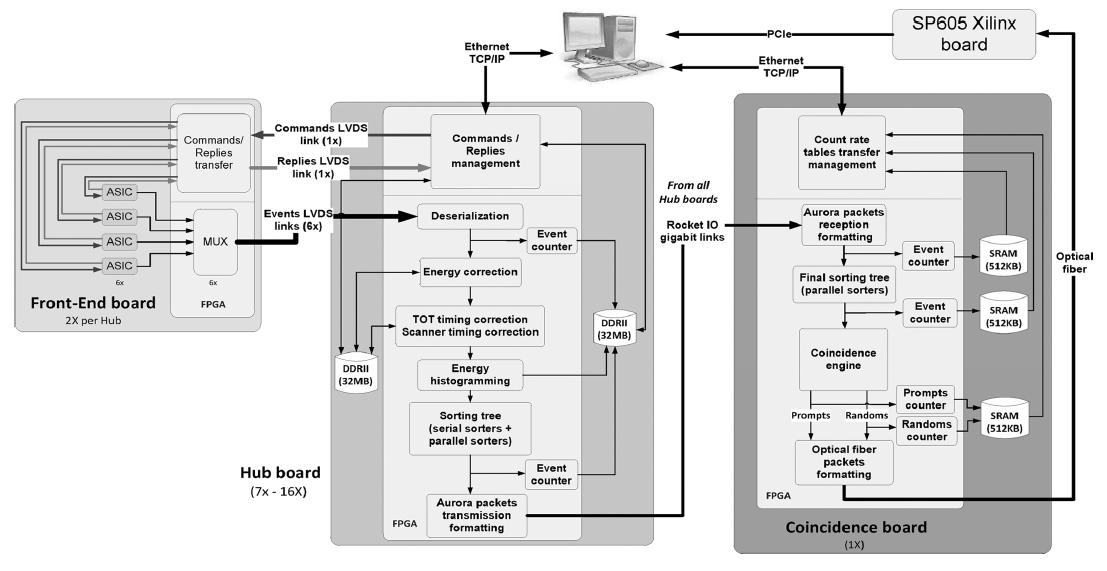
\includegraphics[scale=0.45]{njejimana.png}
		\caption{Diagrama de bloques del sistema de adquisición de datos para LabPET II \cite{Njejimana2013DesignImaging}}
		\label{fig:njejimana}
	\end{figure}
	
\newpage
\section{4D PET}
\label{par:4dpet}
	Otro sistema de referencia es el DAQ para el sistema modular 4D PET \cite{Marcatili2011DevelopmentDetector}. Este dispositivo permite capturar entre 144 a 576 señales provenientes de arreglos matriciales de fotomultiplicadores. Se caracteriza principalmente por poseer una tarjeta madre central, en la cual es posible conectar hasta 18 tarjetas de adquisición. Cada una de estas tarjetas tiene de 8 a 32 canales para adquisición de señales, y su función es capturar, procesar y enviar información a la placa madre. La Figura \ref{fig:marcatili} ilustra la arquitectura de este sistema.
		
	Las señales son capturadas por ASICs (\textit{Application Specific Integrated Circuits}), muestreadas por conversores análogo-digitales y procesadas por una FPGA, mientras que una FPGA principal (etiquetada como Master FPGA) se encarga de controlar a las FPGAs anteriores y de recibir los datos capturados. El procesamiento inicial de las señales se encarga de calcular energía y datos temporales asociados a las partítuclas detectadas, mientras que el procesamiento final relaciona los eventos que hayan sido temporalmente coincidentes enter sí y a su vez calcula el tiempo de vuelvo de las partículas, mediante un conversor de tiempo a señal digital (TDC).
	       	
	Este sistema destaca por su modularidad, la cual permite un fácil escalamiento. En contraste con LabPET II, se utilizan varias placas adquisidoras paralelas en vez de utilizar serialización de datos, permitiendo procesar la información antes de llegar a la FPGA principal. Cabe destacar que esta arquitectura está relacionada con la necesidad de encontrar múltiples eventos simultáneos en distintas ubicaciones, requerimiento que no está presente en el sistema que se planea diseñar para este proyecto de titulación. 
	
	\begin{figure}[h]
		\centering
		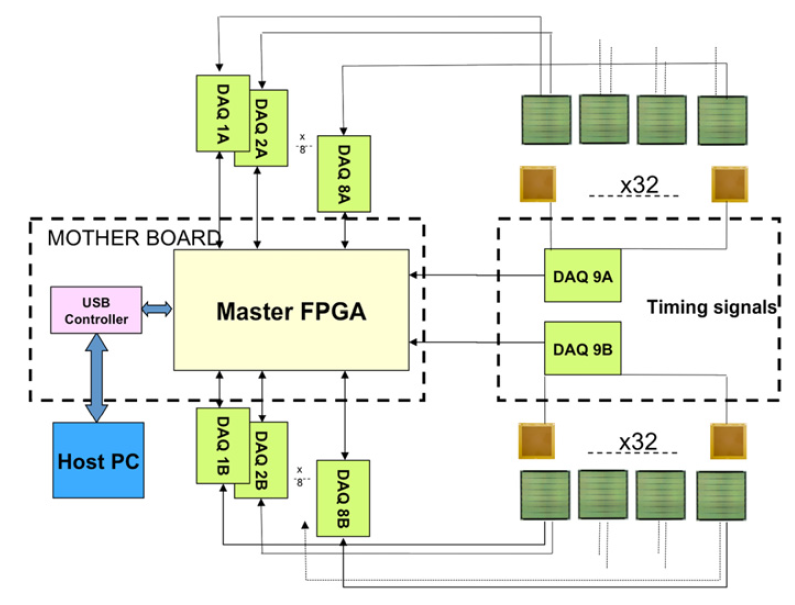
\includegraphics[scale=0.4]{marcatili.png}
		\caption{Diagrama de bloques del sistema de adquisición de datos para Detector PET 4D \cite{Marcatili2011DevelopmentDetector}}
		\label{fig:marcatili}
	\end{figure}
	
\newpage
\section{ATLAS}
	Finalmente, la referencia más importante corresponde al experimento ATLAS \cite{Spieler2012ElectronicsAcquisition}, ya que una de sus etapas utiliza detectores sTGC, mientras que otra de sus etapas utiliza la misma interfaz de lectura que será utilizada en sTGC Minería.

	El experimento ATLAS se encarga de interceptar grupos de partículas provenientes de haces de protones acelerados en el LHC (Large Hadron Collider) en CERN, con el objetivo de estudiar las colisiones de partículas ocurridas a su paso. Las colisiones se generan aproximadamente cada 25$\mu$s\cite{Whiteson2016TheSystem}, y cada colisión pruduce cerca de 23 interacciones con el detector, que junto a otros factores implica cerca de 10$^9$ eventos cada segundo. La tasa de aparición y nivel de energía de estos eventos son las principales razones por las que este detector es tecnológicamente complejo.
	
	El estudio de colisiones tiene como objetivo medir partículas conocidas y deducir la existencia de partículas nuevas. Para lograrlo, es necesario reconstruir las trayectorias e interacciones de todas las partículas medibles mediante múltiples y variados sistemas de detección. Uno de estos sistemas corresponde al Espectrómetro de Muones\cite{Pontecorvo2004TheSpectrometer}, el cual permite determinar la validez de los eventos y trazar la trayectoria de los muones emitidos en las colisiones. 
	
	El Espectrómetro de Muones se compone de múltiples tecnologías de detección diferentes, una de las cuales corresponde a los detectores sTGC ubicados en la Small Wheel, mencionada en la sección \ref{par:smallwheel}. Otra de las tecnologías de detección que componen al Espectrómetro corresponde a los detectores TGC (Thin Gap Chamber), los cuales se diferencian de los detectores sTGC en el tamaño de sus componentes. Los detectores TGC están ubicados en el sector denominado Big Wheel, indicado en la Figura \ref{fig:both-wheels}, y sus datos son obtenidos gracias a una interfaz de lectura llamada ASD (Amplificator-Shaper-Discriminator). Esta inferfaz de lectura, en conjunto con detectores sTGC, da vida al proyecto sTGC Minería en CCTVal, y su funcionamiento será explicado con mayor detalle en el Capítulo \ref{cap:sdet}.
	
	\begin{figure}[h]
		\centering
		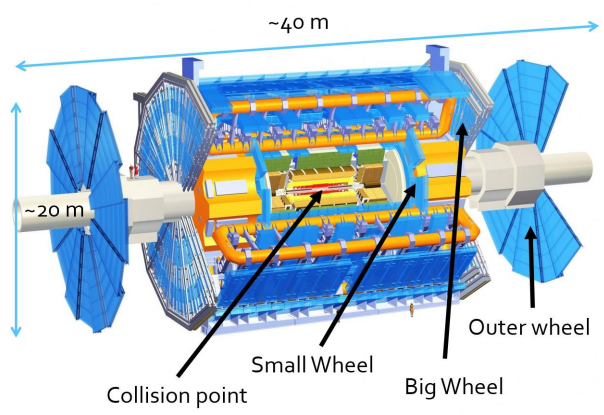
\includegraphics[scale=0.5]{atlas-layout-big-small-wheel.png} 
		\caption{Layout del experimento ATLAS, donde se indica la posiciónde la Small Wheel y la Big Wheel\cite{Formenti2018CERNReport}}
		\label{fig:both-wheels}
	\end{figure}
	
	La Figura \ref{fig:spieler} ilustra el sistema de captura de datos para detectores TGC del Big Wheel en el Espectrómetro de Muones. Los muones son representados con el símbolo $\mu$ y cruzan tres capas de detectores TGC, cada una de las cuales cuenta con sus interfaces de lectura ASD. Los bloques posteriores se encargan de pre-procesar los pulsos capturados y entregarlos a las posteriores etapas de lectura y de selección de eventos.
	
	\begin{figure}[h]
		\centering
		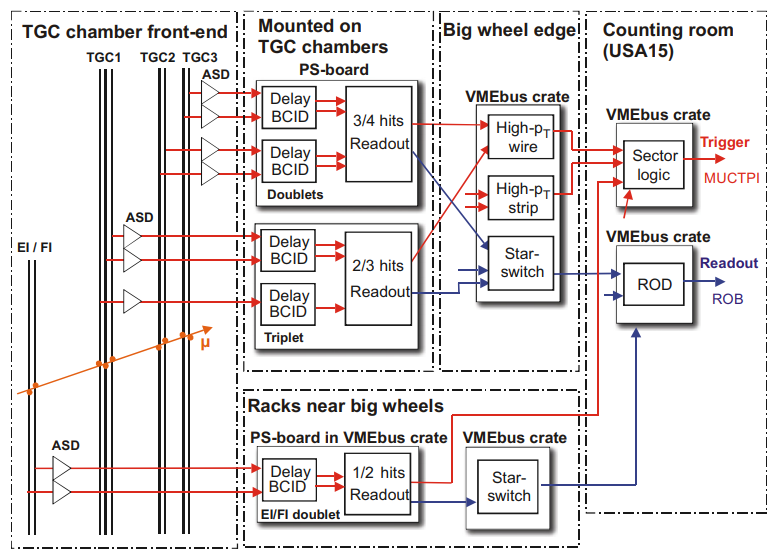
\includegraphics[scale=0.6]{spieler.png}
		\caption{Diagrama de la interfaz de captura para detectores de muones TGC \cite{Spieler2012ElectronicsAcquisition}. Los muones se representan con el símbolo $\mu$. Existen 3 capas de detectores, por lo tanto se observan 3 bloques que incluyen retardos, selección y captura de los pulsos.}
		\label{fig:spieler}
	\end{figure}

	En ATLAS, la selección de eventos a ser estudiados se lleva a cabo en dos etapas. La primera de ellas, llamada \textit{Level 1 Trigger}, involucra al Espectrómetro de Muones y calorímetros. La segunda etapa involucra algoritmos distribuidos en varios computadores y se le conoce como \textit{High-level Trigger}. La Figura \ref{fig:colombo} ilustra ambas etapas en paralelo a los sistemas de lectura de datos. El sistema de lectura de datos ilustrado en \ref{fig:spieler} corresponde al cuadro amarillo ubicado en la esquina superior derecha de la Figura \ref{fig:colombo}, etiquetado como \textit{Muon}. Si el Level 1 Trigger aprueba un evento detectado por el Espectrómetro y los calorímetros, entonces inicia la adquisición de estos datos en la tarjeta de lectura (etiquetada como \textit{Readout System} en la Figura \ref{fig:colombo}). Además, el Level 1 Trigger envía información sobre regiones de interés a analizar, con el fin de llevar a cabo la segunda etapa de selección (\textit{High-Level Trigger}). Esta segunda etapa de selección utiliza software distribuido en cerca de 2000 computadores conectados a una red Ethernet y filtra eventos en función a muestras de datos pertenecientes a las regiones de interés calculadas por el Level 1 Trigger\cite{Colombo2015Data-flowCase}. Finalmente, los eventos seleccionados son trasferidos y  almacenados en los bancos de datos del centro de investigación.
	
	\begin{figure}[h]
		\centering
		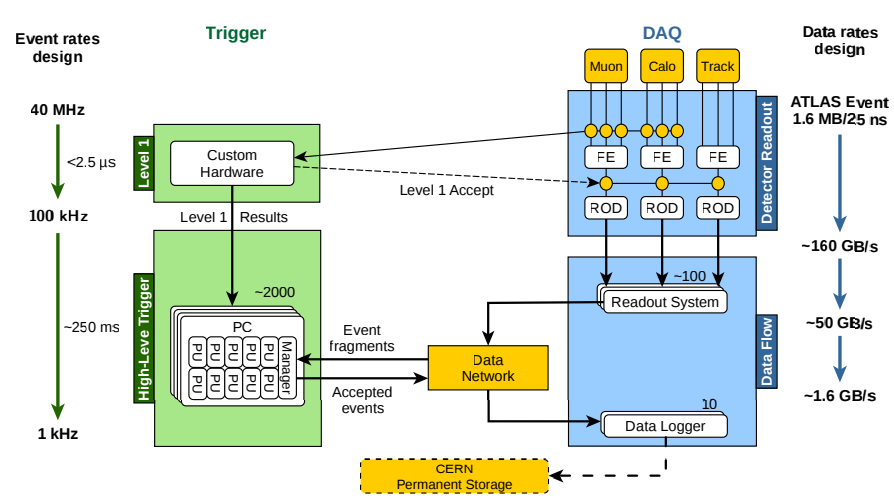
\includegraphics[scale=0.56]{colombo.png}
		\caption{Diagrama del sistema de disparo y adquisición de datos en el experimento ATLAS. \cite{Colombo2015Data-flowCase}}
		\label{fig:colombo}
	\end{figure}
	
	Entrando aún más en detalle respecto a la Figura \ref{fig:colombo}, el verdadero sistema de adquisición de datos en ATLAS es un software distribuido en red\cite{Whiteson2016TheSystem}, capaz de discriminar, procesar y transferir los eventos seleccionados hacia los bancos de almacenamiento de datos. El sistema de lectura (\textit{Readout System}), en conjunto con el Level 1 Trigger, solo sería un equivalente a una interfaz de captura muy sofisticada. Para el caso de esta memoria de titulación, el Readout System del experimento ATLAS sería comparable, en términos de sus niveles de complejidad y de los bloques lógicos que los componen, al sistema de adquisición de datos que se desea diseñar para sTGC Minería.
	
	El Readout System de ATLAS consiste en una tarjeta llamada ROBIN, compuesta de buffers, chips de comunicación, memoria flash, un procesador y una FPGA, como se ilustra en la Figura \ref{fig:whiteson}
	
	\begin{figure}[h]
		\centering
		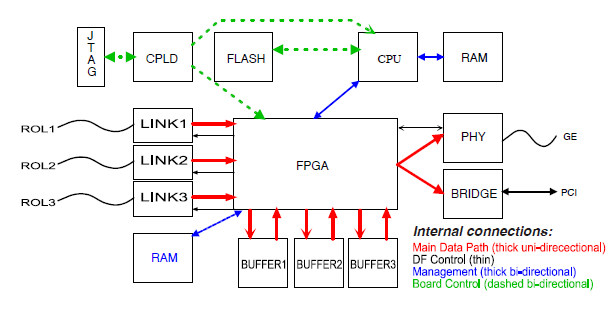
\includegraphics[scale=0.7]{whiteson.png}
		\caption{Diagrama de la tarjeta de lectura ROBIN en ATLAS \cite{Whiteson2016TheSystem}.}
		\label{fig:whiteson}
	\end{figure}
	
	La lógica implementada en la FPGA se ilustra en la Figura \ref{fig:whiteson2}. Se observa que su labor es principalmente controlar los buffers de datos, traspasar los eventos captados hacia la siguiente etapa y eliminar los datos descartados por la señal de disparo de alto nivel.
	
	\begin{figure}[h]
		\centering
		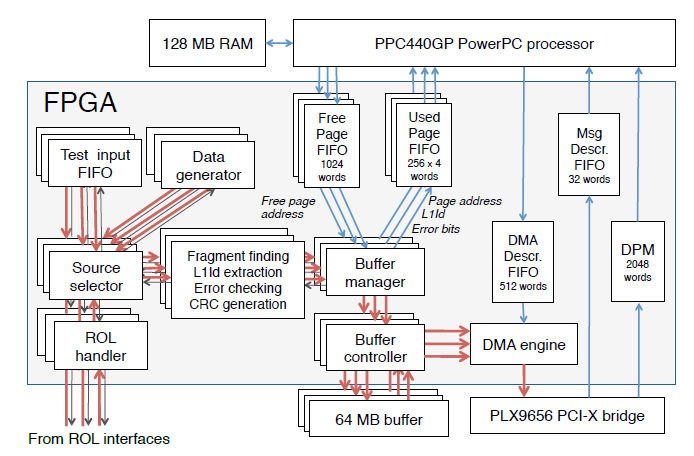
\includegraphics[scale=0.7]{whiteson2.png}
		\caption{Diagrama de bloques de la FPGA en ROBIN \cite{Whiteson2016TheSystem}.}
		\label{fig:whiteson2}
	\end{figure}
	
	\newpage
	Si bien ATLAS es un proyecto con detectores comparativamente más complejos que los descritros en las secciones \ref{par:labpet} y \ref{par:4dpet}, ATLAS presenta elementos comunes con ellos es su composición, sobretodo en cuanto a la utilización de ASICs y FPGAs para captura y control de los datos adquiridos. ATLAS se asemeja funcionalmente al 4D PET, en el sentido de implementar múltiples instancias de hardware equivalente, para así lograr manejar mayor cantidad de datos y brindar mayor control en cada uno de ellos. El fuerte de ATLAS radica en su conectividad en red y sistemas distribuidos, necesarios para la gran cantidad de datos simultáneos que deben ser procesados.


\section{Discusión sobre alternativas existentes}
	Es claro que la tendencia en desarrollo de sistemas de adquisicón es la utilización de ASICs en etapas de primera lectura, mientras que se utilizan FPGAs en etapas de manejo de datos y preprocesamiento, principalmente debido a la magnitud temporal de las señales, a la alta necesidad de precisión en su sincronización, y a la gran cantidad de señales de entrada que deben ser atendidas.
	
	Los elementos más utilizados y recomendados a implementar son los buffers de almacenamiento, principalmente para ajustar la tasa de transmisión de datos de la captura hacia las siguientes etapas de procesamiento, que suelen ser más lentas. En el sistema que se planea diseñar esto no es un problema, ya que la tasa de eventos es muy baja en comparación a los detectores estudiados. Aún así, los buffers pueden ser útiles para el escalamiento de los detectores en el futuro.
	
	El concepto de serialización de datos estuvo principalmente presente en el detector LabPET II. Es pertinente considerarlo, sobretodo para el escalamiento del detector de muones. En caso de requerir cubrir un área mayor o con varias capas superpuestas de detectores, será necesario captar mayor cantidad de señales. Es allí donde se debe decidir si es recomendable comenzar con serialización de datos o con paralelismo de hardware.% Además, dado que es necesario tener noción del tiempo de ocurrencia de los eventos, podría asociarse este dato a cada pulso, facilitando la implementación de serialización de datos. Esto no sería una desventaja, ya que no existe real necesidad de procesar datos de manera rápida y simultanea, reduciendo costos en hardware, pero aumentando esfuerzos de ingeniería.
	
	%Para el caso de pre-procesamiento, selección, formateo y transmisión de datos se puede considerar agregar procesadores dedicados en conjunto con la FPGA principal, que si bien no fueron encontrados textualmente en los ejemplos indicados, sí pueden ser de utilidad, sobretodo dada la existencias de chips que incluyen FPGA en conjunto con procesadores, como los SoC (\textit{System on Chip}) Zynq.
	
	% Finalmente, puede ser interesante incluir métodos de TDC para conversión de la señal digital generada por la placa acondicionadora ASD. La duración de esta señal tiene relación con la amplitud y la energía de los pulsos analógicos captados, lo que podría ser muestreado con una implementación similar a la indicada en \cite{Arpin2010AResources}.
	
	En resumen, es conveniente diseñar el sistema en una FPGA dedicada a la adquisición de datos, incluyendo buffers de almacenamiento para los eventos capturados y replicando este sistema para cada detector adicional.
	

\newpage
\thispagestyle{empty}
\cleardoublepage

\chapter{Arquitectura propuesta}
\label{cap:arq}
En el capítulo Estado del Arte para Proyecto de Titulación \cite{Gonzalez2020EstadoTitulacion} se compararon tres sistemas diferentes para la implementación de adquisición de datos para física de partículas. En ellos destacan aspectos comunes de implementación: etapas de detección de eventos, memorias para almacenamiento temporal, procesamiento de los datos y la utilización de FPGA como herramienta principal para la implementación del hardware.



\section{Alternativas de Solución}
\subsection*{Esquema General}
Tal como se ha planteado en informes anteriores, el esquema básico a implementar es el indicado en la figura \ref{fig:diagrama}. Se requieren al menos tres etapas esenciales: discriminar, procesar y analizar. Discriminar se refiere a distinguir entre aquellos eventos que corresponden un muón de aquellos que no, descartando estos últimos. Procesar implica utilizar los pulsos escogidos, formar una estructura que los relacione como un solo evento y posiblemente incluir información de ellos, como una marca temporal y la duración de los pulsos captados en dicho evento. 

La etapa de análisis implica mayor complejidad y puede extenderse para abarcar distintos niveles. El análisis más básico implica leer un evento e inferir la región del detector que fue excitada por el paso del muón. Niveles siguientes implicarían estimar la energía del muón, incluir mayor precisión espacial, correlacionar con eventos anteriores o incluso trazar la trayectoria  del paso de la partícula al superponer los datos de eventos originados en otros detectores.

\newpage
\subsection*{Requisitos}
Las alternativas aquí propuestas deberán cumplir con las especificaciones mínimas necesarias para captar los pulsos digitales provenientes del detector de muones. Estos requisitos son los siguientes:

\begin{itemize}
	\item Se debe contar con al menos 32 pares de entradas bajo el estándar LVDS, con el fin de conectar al menos 2 tarjetas ASD (Amplificator Shaper Discriminator) utilizadas cada una como la interfaz de detectores de 16 canales.
	\item Es importante contar con un reloj presente o sintetizable de una frecuencia mayor a 100[MHz], lo más cercano a 1[GHz] posible, con el fin de captar la duración de los pulsos y el momento de aparición de un evento con la mayor precisión disponible.
	\item Se debe considerar que la señal de disparo que entrará al sistema estará desfasada cerca de 100[ns] respecto al paso real de los muones por el detector, siendo necesaria la implementación de delays para las señales capturadas o un sistema capaz de distinguir la ocurrencia de eventos y disparos en el tiempo.
	\item  Se debe tener la capacidad de mantener señales sincronizadas, guardar información en memorias temporales y llevar cuenta del transcurso del tiempo entre eventos.
	\item Es requisito que la implementación de la alternativa permita escalamiento para agregar nuevos detectores adyacentes con el fin de aumentar el área de prueba, así como también sincronizarse con detectores paralelos para trazar trayectorias de las partículas captadas.
\end{itemize}

En cuanto a los requisitos de tiempo y reloj de operación anteriormente indicados, estos se deben esencialmente a que la duración de un pulso digital proveniente de un detector podría estar entre 1[ns] y 40[ns]\cite{1999ATLASICs}. Este ancho de pulso tiene correlación con la amplitud del pulso análogo original y el error en su medición implicará menor precisión en la estimación de esta variable.

Respecto a la tasa de aparición de pulsos consecutivos, es poco probable que ocurran eventos simultáneos o cercanos. Se espera que la tasa de muones por centímetro cuadrado sea de un muón por minuto, lo que en los $15[cm^2]$ representados por una señal de detector implicaría cerca de 15 muones por minuto o $2,5*10^{10}$ muones cada 100 [ns], lo que se traduce a una muy baja probabilidad de eventos simultáneos o incluso cercanos. De hecho, la tasa de detección de muones puede disminuir estando bajo tierra y se planea que la toma de una muongrafía conlleve un tiempo prolongado de exposición a rayos cósmicos. Esto conduce a la conclusión de que ignorar posibles eventos simultáneos o adyacentes no tendrá implicancias significativas en los resultados de la muongrafía final.

%\par Dicho lo anterior y planteadas las bases para el desarrollo de alternativas, se presentan a continuación 4 opciones para desarrollar el proyecto de titulación "Sistema de Adquisición de Datos para Detectores de Muones".
%
%
%\newpage
%\subsection{Digitizer}
%Como primera alternativa, se propone la utilización de Digitizers. Estos aparatos son equipos digitalizadores de múltiples canales que permiten guardar en un computador la información de los pulsos captados.
%\par El laboratorio en el cual se desarrolla este proyecto cuenta con digitalizadores CAEN modelo DT5730 (8 canales, 500[MS/s] y 2Vpp de rango de entrada) y modelo DT5740 (32 canales, 62,5[MS/s] y 2Vpp de rango de entrada). 
%\par De los dos equipos considerados, es razonable utilizar el DT5740. Este es capaz de leer al menos 32 canales, suficiente para trabajar con dos detectores de 16 señales. Dada su baja tasa de muestreo, se dificulta la opción de cuantificar el ancho de los pulsos captados, por lo que solo sería fiable la detección posición de muones. Aún así, podría existir error en la sincronización del disparo respecto a los pulsos captados en máximo 17[ns] debido a la baja tasa de muestreo.
%
%\par Adicionalmente a la utilización del equipo digitalizador, se hace necesaria la confección de una interfaz que adapte las señales de tipo LVDS provenientes del acondicionador de señales (ASD) hacia un voltaje legible por el digitizer, el cual podría ser en standard TTL 3.3[V] o CMOS. Tendrá que incluir también lineas o circuitos integrados de retardo para cada una de las señales captadas, del orden de 100[ns] para ser sincrónica con la señal de disparo. La salida de esta nueva tarjeta tendrá que conectarse al digitalizador con cable coaxial de $50[\Omega]$, idealmente de conector LEMO a conector MCX, existentes en el laboratorio y exigido por el digitalizador. La interconexión de esta placa con el resto de los equipos se ilustra en la figura \ref{fig:digitizer1}.
%
%\begin{figure}[H]
%	\centering
%	\includegraphics[scale=1]{imagenes/digitizer1.pdf}
%	\caption{Diagrama de conexiones utilizando un digitalizador CAEN DT7540 y un solo detector de muones. La señal de disparo se encuentra disponible en formato LVDS y TTL.}
%	\label{fig:digitizer1}
%\end{figure}
%
%
%\par Lo descrito anteriormente correspondería a la etapa de captura y discriminación. Para la etapa de procesamiento será necesaria la utilización de software programado en un computador para generar estructuras de datos con información pertinente para el análisis y luego para la implementación del análisis de los eventos captados. La estructura base para este software se ilustra en la figura \ref{fig:digitizer2}
%
%\begin{figure}[H]
%	\centering
%	\includegraphics[scale=1]{imagenes/digitizer2.pdf}
%	\caption{Diagrama de bloques del software, utilizando un digitalizador CAEN DT7540. El módulo de control se encuentra implementado y disponible, basado en librerías del fabricante. Las entradas y salidas de estos bloques son arreglos de datos relacionando la señal con su información. Para el manejo de estos datos se utiliza el framework ROOT\cite{CERN2020ROOT:Framework}. El bloque de formateo ajusta la estructura de datos original para facilitar el procesamiento. El bloque de procesamiento lee los datos determinando el ancho de ellos y asociandolo al canal correspondiente. El bloque de análisis se encarga de estimar la coordenada y eventualmente la energía asociada a cada evento.}
%	\label{fig:digitizer2}
%\end{figure}
%
%
%\par El sistema actualmente descrito es muy similar al procedimiento y configuración circuital utilizados para estudios previos a este proyecto. Se han realizado pruebas al detector en crudo con señales analógicas captadas por digitalizadores de pocos canales, procesando y analizando posteriormente los pulsos para comprobar calidad y factibilidad.
%
%\subsubsection*{Atributos}
%\begin{itemize}
%	\item \textbf{Simplicidad:} Media. Requiere la fabricación de una PCB de interfaz y la integración de 3 aparatos distintos (Digitalizador, interfaz y computador).
%	\item \textbf{Desempeño:} Bajo. Baja tasa de muestreo.
%	\item \textbf{Disponibilidad:} Media. Se cuenta con un digitalizador, pero no está disponible una interfaz LVDS a TTL.
%	\item \textbf{Economía:} Baja. El costo de digitalizadores adicionales podría superar los US\$1000.
%\end{itemize}
%
%\subsubsection*{Ventajas}
%\begin{itemize}
%	\item Planificación simplificada.
%	\item Etapas claras.
%	\item Adaptable en etapa de software.
%\end{itemize}
%
%
%\subsubsection*{Desventajas}
%\begin{itemize}
%	\item Baja tasa de muestreo.
%	\item Alto costo.
%	\item Poco práctico.
%	\item Difícil escalamiento.
%	\item Requiere fabricación de hardware adicional.
%\end{itemize}

%\newpage
%\subsection{Microcontrolador}
%\label{sec:micro}
%\par Una alternativa común en el rubro de la electrónica es el uso de microcontroladores. Destacan por su versatilidad pero no son aplicables a todos los casos. Para esta alternativa de solución se buscaron placas de desarrollo con microcontroladores con un número de entradas y frecuencia de reloj razonable, pero no fue posible encontrar uno que cumpliera con todo lo necesario. 
%\par En afán de utilizar un microcontrolador como alternativa comparativa, se plantea la posibilidad de utilizar múltiples unidades de manera paralela, logrando satisfacer el requisito de cantidad de señales.
%
%\par Dado que se requiere trabajar con señales LVDS, se vuelve necesario incluir conversores LVDS-TTL en esta alternativa de solución. Para captarlas y medirlas sería necesaria la existencias de conversores análogo-digitales (ADC) para muestrear las señales. Si bien son originalmente de naturaleza digital, no es posible captarlas y muestrearlas con facilidad sin la utilización de ADCs.
%
%\par Para trabajar con la señal de disparo desfasada, se pueden utilizar memorias incluidas en las placas de desarrollo para almacenar los pulsos en orden de llegada mientras se espera por una señal de disparo. En el momento de su llegada, es posible buscar en memoria los pulsos que hayan sido muestreados en un tiempo atrás equivalente al desfase del disparo y estructurar la información como un nuevo evento válido.
%
%\par Dada la baja frecuencia de reloj que se encuentra comúnmente en las tarjetas de desarrollo de microcontroladores, se dificulta la operación y precisión del sistema. Si bien esto puede mejorar con la frecuencia de muestreo de los ADC, sigue siendo difícil y costoso acercarse a 1[]GSPS].
%
%\par Finalmente, las etapas de procesamiento se pueden ver facilitadas en esta alternativa. La implementación de ellas en un microcontrolador suele ser más intuitiva y óptima dada su naturaleza para trabajar operaciones matemáticas. Por otro lado, sincronizar los eventos y los datos entre microcontroladores adyacentes puede ser un desafío considerable. En las figuras \ref{fig:microcontrolador1}, \ref{fig:microcontrolador2}, y \ref{fig:microcontrolador3} se ilustra esta propuesta en base a un microcontrolador.
%
%\begin{figure}[H]
%	\centering
%	\includegraphics[scale=1]{imagenes/microcontrolador1.pdf}
%	\caption{Diagrama de bloques utilizando microcontroladores como alternativa de solución con un solo detector. Dado que el numero de puertos es bajo, puede ser necesario utilizar dos microcontroladores por cada detector. Además, se hace necesario un microcontrolador adicional para captar y relacionar los eventos de las etapas anteriores, unificándolos en un solo evento.}
%	\label{fig:microcontrolador1}
%\end{figure}
%
%\begin{figure}[H]
%	\centering
%	\includegraphics[scale=1]{imagenes/microcontrolador2.pdf}
%	\caption{Representación en diagramas de bloques de los elementos internos de uno de los microcontroladores iniciales. Se encarga de captar la mitad de los pulsos originados por un detector. El bloque ADC muestrea los pulso en el tiempo, almacenándolos en una cola de datos FIFO. Un controlador de esta cola determina el avance o descarte de datos en función de las señales de disparo captadas. El bloque sincronizador apoya la operación de dos microcontroladores simultáneos, asegurándose que ambos capten los mismos eventos. El estructurador de datos da forma a la información, asociando duración de pulso a cada uno de los canales captados, para luego enviarlo a la siguiente etapa mediante comunicación serial.}
%	\label{fig:microcontrolador2}
%\end{figure}
%
%\begin{figure}[H]
%	\centering
%	\includegraphics[scale=1]{imagenes/microcontrolador3.pdf}
%	\caption{Representación en diagramas de bloques de los elementos internos del microcontrolador final. Se encarga de unificar eventos de dos microcontroladores distintos, incluso pudiendo escalarse a unificar eventos procedentes de más detectores. Aquí existe un segundo bloque estructurador, encargado de unificar, entregando una estructura de igual notación pero mayor tamaño. El bloque de análisis de coordenadas permite la estimación de la coordenada por la cual ha pasado la partícula y eventualmente la energía asociada, para luego enviar esta información a una etapa siguiente de análisis profundo mediante comunicación serial.}
%	\label{fig:microcontrolador3}
%\end{figure}
%
%
%\newpage
%\subsubsection*{Atributos}
%\begin{itemize}
%	\item \textbf{Simplicidad: } Baja. Gran cantidad de dispositivos.
%	\item \textbf{Desempeño: } Bajo. Bajas tasas de muestreo y operación.
%	\item \textbf{Disponibilidad: } Baja. Todos los materiales tendrían que ser adquiridos.
%	\item \textbf{Economía: } Baja, poco económico. Si bien las tarjetas de desarrollo pueden ser de bajo costo, se necesitan varias y se agregan componentes extra que aumentan el costo considerablemente.
%\end{itemize}
%
%\subsubsection*{Ventajas}
%\begin{itemize}
%	\item Escalable.
%	\item Tecnologías muy conocidas.
%	\item Facilita el análisis y operaciones matemáticas.
%\end{itemize}
%
%
%\subsubsection*{Desventajas}
%\begin{itemize}
%	\item Costoso.
%	\item Bajo desempeño.
%	\item Varias fuentes de error, dada su complejidad.
%	\item Poca disponibilidad de los materiales y hardware necesario.
%\end{itemize}

%\newpage
%\subsection{CPLD}
%\par Otra alternativa de solución consiste en describir módulos de hardware en una CPLD (Complex Programable Logic Device). Estos dispositivos tienen la ventaja de ser de bajo costo, pero con la condición de contar con pocos recursos lógicos para su operación.
%\par Contar con la posibilidad de describir el hardware en su interior facilita la implementación del sistema, logrando resultados mejor adaptados al problema real.
%\par Una tarjeta de desarrollo para CPLD es la Lattice MACH X02\cite{Semiconductor2017DS1035Sheet}. Esta tarjeta cuenta con cerca de 7000 LUTs (Look-up tables), cerca de 250kb de memoria RAM, relojes sintetizables de hasta 400MHz y particularmente 114 puertos LVDS, suficientes para conectar al menos dos detectores sin tarjetas intermedias con hardware adicional. Esto no quita que se requiera de una tarjeta o adaptador para conectar las señales del detector a la tarjeta de desarrollo.
%
%\par Las grandes desventajas de esta tarjeta son sus escasos recursos disponibles y nulos periféricos. Si bien sus frecuencias de reloj son destacables, aún pueden ser mejores en otras alternativas.
%
%\par La implementación propuesta para esta alternativa rescata elementos de alternativas anteriores, en especial para el tratamiento del desfase de la señal de disparo, rescatando eventos anteriormente guardados en memoria. Su mayor frecuencia de reloj permite el tratamiento de las señales con una precisión mayor y más razonable, teniendo errores de cerca de 2.5[ns] en el arribo de señales y en la medición de anchos de pulso. Las figuras \ref{fig:cpld1}, \ref{fig:cpld2}, \ref{fig:cpld3} reflejan la solución propuesta.
%
%\par Para la etapa de análisis se hace necesario el apoyo de un computador que tome los paquetes de eventos procesados por la CPLD y sea capaz de extraer la información de interés.
%
%\begin{figure}[H]
%	\centering
%	\includegraphics[scale=1]{imagenes/cpld1}
%	\caption{Diagrama de bloques utilizando una CPLD como alternativa de solución.}
%	\label{fig:cpld1}
%\end{figure}
%
%
%
%\begin{figure}[H]
%	\centering
%	\includegraphics[scale=1]{imagenes/cpld2}
%	\caption{Diagrama de bloques de la lógica interna descrita para la CPLD. Similar a la estructura interna propuesta para los microcontroladores iniciales de la figura \ref{fig:microcontrolador2}. Aquí no existe sincronización explicita con una segunda CPLD ya que solo se utiliza una por detector. El estructurador de datos cumple la misma función de asociar duración de pulso a cada canal medido del evento. Las etapas de análisis no se realizan y se delegan a una etapa posterior.}
%	\label{fig:cpld2}
%\end{figure}
%
%\newpage
%\begin{figure}[H]
%	\centering
%	\includegraphics[scale=1]{imagenes/cpld3}
%	\caption{Representación del software presente en un computador de apoyo. Su estructura y funcionamiento cumple la misma idea de lo planteado para la primera alternativa de solución, como ilustra la figura \ref{fig:digitizer2}.}
%	\label{fig:cpld3}
%\end{figure}
%
%
%\par En cuanto al escalamiento, sería factible utilizar una CPLD cada dos detectores. Aún así, se debería tener la precaución de optimizar el hardware a un nivel tal que los recursos sean suficientes para la implementación.
%
%\subsubsection*{Atributos}
%\begin{itemize}
%	\item \textbf{Simplicidad:  } Alta. Pocos dispositivos involucrados.
%	\item \textbf{Desempeño:}  Medio. Escasos recursos lógicos y periféricos.
%	\item \textbf{Disponibilidad:}  Alta. Se cuenta con una de estas tarjetas en el laboratorio.
%	\item \textbf{Economía: } Alta. Una de estas tarjetas tiene un valor cercano a los US\$30.
%\end{itemize}
%
%\subsubsection*{Ventajas}
%\begin{itemize}
%	\item Muy económica.
%	\item Alta frecuencia de reloj comparada con alternativas anteriores.
%	\item Cuenta con puertos LVDS.
%	\item Escalable.
%\end{itemize}
%
%
%\subsubsection*{Desventajas}
%\begin{itemize}
%	\item Pocos recursos lógicos disponibles.
%	\item Escasa memoria para almacenar pulsos y eventos
%	\item Pocos periféricos, prácticamente solo cuenta con comunicación serial.
%	\item Se requiere confeccionar un adaptador para conectar el detector con la tarjeta de desarrollo.
%\end{itemize}

\newpage
\subsection{FPGA}
La alternativa más utilizada en el rubro es la FPGA. Esta ha sido la herramienta que se ha visto con mayor frecuencia en proyectos relativos a física de partículas y adquisición de datos. 
Las FPGA cuentan con una cantidad significativa de recursos y periféricos. Incluyen además hardware dedicado para comunicación, serialización y almacenamiento de datos. Incluso suelen incluir CPLDs en las placas que las albergan. Una desventaja conocida corresponde a que se basan en memorias volátiles, por lo que el hardware descrito se debe reconfigurar cada vez que se enciende, y los datos importantes deben ser almacenados en memorias externas.

Para esta alternativa se propone el uso de la tarjeta de desarrollo Trenz TR0712 \cite{TrenzElectronic2019TR07012Wiki} montada en una placa TR0703 \cite{TrenzElectronic2019TR0703Wiki}. Esta tarjeta en su conjunto se basa en una FPGA Xilinx Artix 7 \cite{Xilinx20107DS180} de cerca de 16.000 celdas lógicas, incluyendo además chips de memoria RAM, reloj de 20[MHz] con hasta 600[MHz] sintetizables, comunicación Ethernet y por supuesto puertos LVDS suficientes para conectar al menos 2 detectores.

Si bien esta tarjeta cuenta con puertos LVDS, será necesario confeccionar un adaptador para conectar las señales del detector hacia la placa Trenz.

%En esta alternativa se rescatan los diseños de hardware mencionados con anterioridad, con la holgura de que existen recursos suficientes para implementar los bloques indicados. Incluso se evalúa incluir parte del análisis dentro de la FPGA y no destinarla a un computador en su totalidad.

La frecuencia de reloj que puede alcanzar esta tarjeta es mucho mayor que cualquiera de las anteriores, siendo entonces la que permite tener mayor precisión en términos de tiempo, sobretodo para determinar la duración de los pulsos provenientes del detector.

La idea en esta alternativa de solución es guardar los datos en memoria temporal hasta la llegada de una señal de disparo. Un módulo que maneja la memoria será el encargado de tomar los pulsos correspondientes al disparo recibido y liberar la memoria de aquellos datos ya leídos u obsoletos, entregando la información útil a una siguiente etapa. Los pulsos aceptados serán entonces relacionados como parte de un mismo eventos y se estimará la duración de estos, generando y guardando así un arreglo de datos con identificador de pulso y duración. La última etapa se encargará de efectuar una operación capaz de determinar la posición del evento a partir de las duraciones medidas y los pulsos detectados, comunicando así un arreglo básico y preprocesado que incluya posición y magnitud aproximada.

\par Se espera que para lograr el escalamiento se incluya una señal para mantener la lectura de eventos sincronizada entre distintas FPGA. Además, se deberá incluir un modulo de comunicación para entregar la información captada a una etapa posterior con un análisis más detallado, encargado de reunir todos los eventos de diferentes FPGAs.

\newpage
\par Las figuras \ref{fig:fpga1} \ref{fig:fpga2} ilustran conexiones y bloques a implementar en esta alternativa de solución.

\begin{figure}[H]
	\centering
	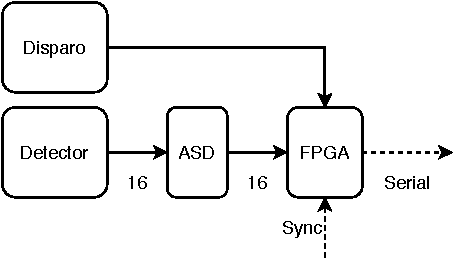
\includegraphics[scale=1]{imagenes/fpga1.pdf}
	\caption{Diagrama de bloques utilizando una FPGA como alternativa de solución. Se indica una salida serial para transmitir los resultados del análisis básico a algún procesador o memoria de alguna etapa posterior. La señal de sincronización, inspirada en la alternativa \ref{sec:micro} tiene como objetivo sincronizar la recolección y procesamiento de eventos, para que estos sean consistentes entre detectores.}
	\label{fig:fpga1}
\end{figure}

\begin{figure}[H]
	\centering
	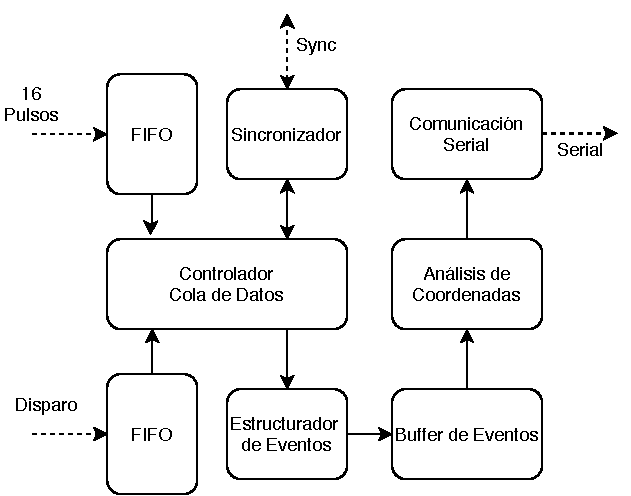
\includegraphics[scale=1]{imagenes/fpga2.pdf}
	\caption{Representación de la lógica interna de la FPGA. Se agrega una cola de datos para las señales de disparo y una memoria de almacenamiento temporal para los eventos ya estructurados. Ambas implementaciones permiten tener mejor control del flujo de datos, evitando perdidas y asegurando sincronía a pesar de que la lectura de la información sea eventualmente más lenta que la captura de pulsos. Los bloques controlador, estructurador y análisis cumplen las mismas funciones mencionadas en alternativas anteriores: aceptar o descartar pulsos, cuantificar anchos de pulso a  los canales asociados y determinar coordenada del cruce de un muón respectivamente.}
	\label{fig:fpga2}
\end{figure}

\newpage
\subsubsection*{Atributos}
\begin{itemize}
	\item \textbf{Simplicidad:}  Media. Gran cantidad del sistema concentrado en una sola placa, pero aumenta la dificultad en la descripción de hardware.
	\item \textbf{Desempeño:}  Alto. Gran cantidad de recursos lógicos, de almacenaiento y de frecuencia de operación.
	\item \textbf{Disponibilidad: } Alta. Se cuenta con una en el laboratorio.
	\item \textbf{Economía: } Media. Una tarjeta de desarrollo de este estilo tiene un costo de aproximadamente US\$400.
\end{itemize}

\subsubsection*{Ventajas}
\begin{itemize}
	\item Gran cantidad del sistema concentrado en una sola placa.
	\item Escalable
	\item Cuenta con puertos LVDS
	\item Alta densidad de recursos lógicos
	\item Dispone de memoria suficiente para almacenar eventos
	\item Posee una alta frecuencia de reloj sintetizable, mejorando precisión temporal.
	\item Placa con muy buena documentación.
\end{itemize}


\subsubsection*{Desventajas}
\begin{itemize}
	\item Se requiere confeccionar un adaptador para conectar el detector con la tarjeta de desarrollo.
	\item Se complica el diseño y la implementación del hardware.
\end{itemize}




%\newpage
%\section{Conclusiones}
%\par Luego de estudiar cuatro alternativas de solución, es posible aseverar que una FPGA cuenta con la mayor capacidad para cumplir con los objetivos de este proyecto.
%\par Si bien otras alternativas pueden tener ventajas en cuanto a precio, una FPGA simplifica algunas labores y da la holgura necesaria para implementar el sistema descrito.
%\par Una quinta alternativa muy interesante es la utilización de una FPGA en conjunto con un procesador, como es el caso de las Zynq, mencionadas en informes anteriores. Estos dispositivos no fueron considerados ya que en el laboratorio no se encuentran disponibles tarjetas de desarrollo que cumplan con las especificaciones planteadas, particularmente con el número de puertos LVDS accesibles y necesarios para la confección del detector.
%\par Otra alternativa descartada ha sido la aplicación de TDC (Time to Digital Converter)\cite{Arpin2010AResources}, que si bien permitiría mejorar la resolución temporal del sistema, implica un desafío ingenieril y de recursos a una escala un tanto mayor.
%\par Estas dos últimas propuestas quedan disponibles para ser implementadas en iteraciones posteriores, una vez que se tenga certeza del funcionamiento básico requerido que el actual proyecto plantea.


%%%%%%%%%%%%%%%%%%%%%%%%%%%%%

¿Cuáles son las etapas esenciales que un DAQ debe poseer? En esencia se requiere de una primera etapa de interfaz de lectura directamente de los detectores (\textit{Readout}), las cuales suelen poseer amplificadores, modeladores de pulsos, memorias y digitalizadores. Una segunda etapa suele consistir en el preprocesamiento de las señales, extrayendo la información básica y formando estructuras de datos pertinentes. Finalmente, está la etapa de procesamiento fuera del detector, donde se realiza el análisis e interpretación de los datos.

En este proyecto de titulación, la primera etapa la lleva a cabo la tarjeta acondicionadora ASD (Amplifier Shaper Discriminator), diseñada para detectores del proyecto ATLAS. Las etapas restantes serán diseñadas pensando en la aplicación específica de este proyecto.

%En el documento ``Alternativas de Solución de Proyecto de Titulación'' se presentaron 4 posibles alternativas para la implementación de un sistema de adquisición de datos para detectores de muones. En cada una de ellas se proponen distintas tecnologías para llevar acabo el mismo fin: Digitizers, Microcontroladores, CPLDs y FPGAs. La figura \ref{fig:diagrama} ilustra la estructura general del sistema de adquisicón de datos.
%
%En el actual documento se presenta el contraste entre las 4 alternativas discutidas con anterioridad, asignando puntaciones a cada una de ellas en base a criterios clave asociados a las características y el diseño del sistema. Los criterios a evaluar son: simplicidad, desempeño, disponibilidad, economía, flexibilidad y documentación. La comparativa que se desarrolla aquí tiene como objetivo definir cuál de las 4 opciones es la mejor alternativa a desarrollar, cumpliendo además con los requisitos principales del proyecto.
%
%La alternativa seleccionada se presenta y detalla a continuación de la comparación de alternativas, planteando sus características principales y justificando la elección realizada.
%\begin{figure}[H]
%    \centering
%    
%    \tikzstyle{externo} = [rectangle, rounded corners, minimum width=2cm, minimum height=1cm,text centered, draw=black, fill=blue!30]
%    \tikzstyle{fpga} = [rectangle, rounded corners, minimum width=3cm, minimum height=2.5cm,text centered, draw=black, fill=green!30]
%    \tikzstyle{flecha} = [thick,->,>=stealth]   
%    
%    \begin{tikzpicture}[node distance=1.5cm]
%
%        \node (disparo) [externo] {Disparo};
%        \node (detector) [externo, below of=disparo] {Detector};
%        \node (asd) [externo, right of=detector, xshift=1cm] {ASD};
%        \node (disc) [fpga, right of=detector, xshift=2.5cm, yshift=-0.5cm, anchor=south west] {Discriminador};
%        \node (pros) [fpga, right of=disc, xshift=2cm] {Procesamiento};
%        \node (res) [fpga, right of=pros, xshift=2cm] {Análisis};
%        
%        \draw [flecha] (disparo) --  (disc.west |- disparo);
%        \draw [flecha] (detector) -- (asd);
%        \draw [flecha] (asd) -- (disc.west |- asd);
%        \draw [flecha] (disc) -- (pros);
%        \draw [flecha] (pros) -- (res);
%
%    \end{tikzpicture}
%
%    \caption{Diagrama de bloques del sistema. En azul se presentan las etapas previas al proyecto que ya se encuentran desarrolladas y sobre las cuales no se tiene control. En verde se ilustran las etapas pendientes y que pueden ser desarrolladas en este proyecto. El disparo corresponde a la señal digital que indica si la partícula detectada es un muón y el ASD es un acondicionador de señal que genera pulsos digitales a partir de los pulsos analógicos captados.}
%    \label{fig:diagrama}
%\end{figure}


%\section{Criterios de Selección}
%\par Para seleccionar la alternativa más adecuada se definieron seis distintos criterios de evaluación, cada uno de los cuales puede obtener un puntaje entre 1 y 10. Los criterios tienen distinta relevancia dentro del proyecto, resultando en que algunos de ellos tengan mayor ponderación respecto a otros. La tabla \ref{tab:criterios} indica el porcentaje de relevancia correspondiente cada criterio de selección. 
%
%\begin{table}[H]
%	\centering
%	\begin{tabular}{|l|c|}
%		\hline
%		\textbf{Criterio de Selección} & \textbf{Porcentaje de Relevancia} \\ \hline
%		Simplicidad & 10\% \\ \hline
%		Desempeño & 35\% \\ \hline
%		Disponibilidad & 25\% \\ \hline
%		Economía & 10\% \\ \hline
%		Flexibilidad & 10\% \\ \hline
%		Documentación & 10\% \\ \hline
%		\textit{Total} & \textit{100\%} \\ \hline
%	\end{tabular}
%	\caption{Porcentaje de relevancia para cada criterio.}
%	\label{tab:criterios}
%\end{table}
%
%\newpage
%\par Se considera como criterio de mayor importancia al \textit{desempeño} estimado de la alternativa, ya que será el aspecto que defina la calidad y funcionamiento del sistema. En segundo lugar de relevancia se ubica la \textit{disponibilidad} de recursos, ya que sin ellos no es posible construir el dispositivo. Los criterios restantes se consideraron menor con ponderación ya que son importantes, pero no cruciales para llevar a cabo el proyecto en su primera versión.
%\par Cada criterio es evaluado con un puntaje de 1 a 10 puntos en una escala indicada en la tabla \ref{tab:escala}. A continuación se detalla cada criterio, incluyendo su descripción y explicando la interpretación de puntaje según la escala mencionada.
%
%\begin{table}[H]
%	\centering
%	\begin{tabular}{lllll}
%		\hline
%		\multicolumn{1}{|c|}{\textbf{Muy Baja}} & \multicolumn{1}{c|}{\textbf{Baja}} & \multicolumn{1}{c|}{\textbf{Media}} & \multicolumn{1}{c|}{\textbf{Alta}} & \multicolumn{1}{c|}{\textbf{Muy Alta}} \\ \hline
%		\multicolumn{1}{|c|}{1 - 2}                 & \multicolumn{1}{c|}{3 - 4}             & \multicolumn{1}{c|}{5 - 6}           & \multicolumn{1}{c|}{7 - 8}           & \multicolumn{1}{c|}{9 - 10}              \\ \hline 
%	\end{tabular}
%	\caption{Tabla de puntajes para criterios de evaluación.}
%	\label{tab:escala}
%\end{table}
%
%\subsection*{Simplicidad}
%\par El criterio de simplicidad se refiere a la dificultad de diseñar, programar, fabricar y ensamblar el sistema descrito en la alternativa evaluada. La máxima simplicidad está indicada con un puntaje 10 y la mínima simplicidad con un puntaje 1. Máxima simplicidad implica conectar elementos sin mayor esfuerzo, prácticamente no programar software y prácticamente no diseñar ni implementar hardware. Mínima simplicidad implicaría dificultad de interconexión entre elementos componentes, debido a sus estándares o cantidad de conexiones presentes, incluyendo software de alta complejidad y prácticamente el desarrollo completo del hardware.
%
%\subsection*{Desempeño}
%La evaluación por desempeño tiene directa relación con los requisitos de diseño asociados al sistema a desarrollar. Estos requisitos son los siguientes:
%
%\begin{itemize}
%	\item Se debe contar con al menos 32 pares de entradas bajo el estándar LVDS, con el fin de conectar al menos 2 tarjetas ASD (Amplificator Shaper Discriminator) utilizadas cada una como la interfaz de detectores de 16 canales.
%	\item Es importante contar con un reloj presente o sintetizable de una frecuencia mayor a 100[MHz], lo más cercano a 1[GHz] posible, con el fin de captar la duración de los pulsos y el momento de aparición de un evento con la mayor precisión disponible.
%	\item Se debe considerar que la señal de disparo que entrará al sistema estará desfasada cerca de 100[ns] respecto al paso real de los muones por el detector, siendo necesaria la implementación de retardos para las señales capturadas o un sistema capaz de distinguir la ocurrencia de eventos y disparos en el tiempo.
%	\item  Se debe tener la capacidad de mantener señales sincronizadas, guardar información en memorias temporales y llevar cuenta del transcurso del tiempo entre eventos.
%	\item Es requisito que la implementación de la alternativa permita escalamiento para agregar nuevos detectores adyacentes con el fin de aumentar el área de prueba, así como también sincronizarse con detectores paralelos para trazar trayectorias de las partículas captadas.
%\end{itemize}
%
%\par Sintetizando estos requisitos, es posible acotarlos a  5 elementos esenciales: número de canales, disponibilidad de puertos LVDS, frecuencia de reloj, implementación o manejo de retardos y recursos de almacenamientos o procesamiento disponibles. La escalabilidad queda implícitamente evaluada con los criterios de simplicidad, economía y flexibilidad.
%
%\par Considerando lo anterior, se le asignará puntaje a este criterio en función de la cantidad de requisitos que cumpla y la calidad con la que sean satisfechos, considerando 10 puntos en caso de cumplir a cabalidad con todos ellos, y asignándole 1 punto en caso de cumplir ninguno.
%
%\subsection*{Disponibilidad}
%\par El criterio de disponibilidad evalúa la presencia inmediata de los materiales necesarios para la implementación del sistema. Pondera la cantidad de elementos necesarios como un total de 10 puntos repartidos en cada uno de los elementos componentes para construir un sistema de adquisición de 32 canales. Si un sistema requiere de 5 elementos discretos, tendrá entonces 10 puntos en caso de contar con la disponibilidad de los 5 elementos necesarios. Si alguno no está disponible y requiere ser adquirido, entonces implicaría un descuento de 2 puntos en dicho ejemplo.
%
%\subsection*{Economía}
%\par El criterio de economía evalúa el precio total de construcción del dispositivo, incluyendo todo el hardware necesario para la discriminación, procesamiento y análisis, sin considerar un computador en las etapas finales de análisis o recolección de información. Este criterio es útil para contrastar la factibilidad de escalamiento. Un sistema muy costoso implicará dificultades para replicarlo.
%\par Su puntaje se asigna considerando cero puntos para un sistema que supere los US\$1000 para implementar 32 canales. Se otorga un máximo de 10 puntos si el sistema tiene un costo menor o igual a US\$60.
%
%\subsection*{Flexibilidad}
%\par La flexibilidad es un criterio que representa qué tan adaptable es el sistema en caso de requerir modificaciones. Puede separarse en tres elementos constitutivos: adquisición, procesamiento y análisis. El puntaje se asigna cualitativamente en función de la flexibilidad de la tecnología involucrada en dicha etapa.
%\par El puntaje máximo del criterio de flexibilidad son 10 puntos, considerando aproximadamente 3.3 puntos como máximo para cada elemento constitutivo.
%
%\subsection*{Documentación}
%\par El criterio de documentación evalúa la disponibilidad de material bibliográfico, tutoriales y ejemplos para la utilización del software y el hardware propio del sistema, así como de las herramientas necesarias para su implementación. Su puntaje se asigna cualitativamente según la misma tabla \ref{tab:escala}.

%\newpage
%\section{Evaluación de Alternativas}
%\label{evaluacion}
%\par A continuación se detallan las evaluaciones para cada una de las 4 alternativas propuestas, incluyendo una breve descripción por cada criterio.
%\subsection{Digitizer}
%\begin{itemize}
%	\item \textbf{Simplicidad:} \textit{5 - Media}. Requiere la fabricación de una PCB de interfaz y la integración de 3 aparatos distintos (Digitalizador, interfaz y computador).
%	\item \textbf{Desempeño:} \textit{4 - Bajo}. Baja tasa de muestreo, 62.5[MS/s].
%	\item \textbf{Disponibilidad:} \textit{2 - Muy Baja}. Se cuenta con un digitalizador, pero no está disponible una interfaz LVDS a TTL ni los retardos necesarios.
%	\item \textbf{Economía:} \textit{1 - Muy Baja}. El costo de  un  digitalizador podría superar los US\$1000.
%	\item \textbf{Flexibilidad:} \textit{5 - Media}. Alta flexibilidad en análisis ya que se realiza en un computador. También existe flexibilidad en la manera de procesar y estructurar los datos obtenidos. No existe suficiente flexibilidad en la manera de tomar muestras.
%	\item \textbf{Documentación:} \textit{6 - Media} Existe documentación, librerías y programas para operar el digitalizador, pero no son las suficientes para tener el dominio total del dispositivo.
%\end{itemize}
%
%\subsection{Microcontrolador}
%\begin{itemize}
%	\item \textbf{Simplicidad: } \textit{2 - Baja}. Gran cantidad de dispositivos, al ser necesario al menos dos microcontroladores por canal y un tercero para unificar datos provenientes de un mismo detector.
%	\item \textbf{Desempeño: } \textit{4 - Bajo}. Bajas tasas de muestreo y operación. Requiere conversores LVDS-TTL y retardos.
%	\item \textbf{Disponibilidad: } \textit{1 - Baja}. Todos los materiales tendrían que ser adquiridos.
%	\item \textbf{Economía: } \textit{6 - Media}, medianamente económico. Si bien las tarjetas de desarrollo pueden ser de bajo costo, se necesitan varias y se agregan componentes extra que aumentan el costo considerablemente. Mejorar la frecuencia de muestreo también incrementa el costo.
%	\item \textbf{Flexibilidad:} \textit{5 - Media}. Alta flexibilidad en análisis y en la manera de procesar y estructurar los datos obtenidos. No existe suficiente flexibilidad en la manera de tomar muestras.
%	\item \textbf{Documentación:} \textit{6 - Media} Existe documentación, librerías y programas de ejemplo, pero queda sujeto a los microcontroladores que eventualmente se escojan.
%\end{itemize}
%
%\newpage
%\subsection{CPLD}
%\begin{itemize}
%	\item \textbf{Simplicidad:} \textit{7 - Alta}. Pocos dispositivos involucrados, solo una CPLD por detector.
%	\item \textbf{Desempeño:}  \textit{7 - Alto}. Escasos recursos lógicos y periféricos, pero alta velocidad de reloj (400MHz máximo), opciones para manejar ratardos y cuenta con puertos LVDS.
%	\item \textbf{Disponibilidad:} \textit{9 - Alta}. Se cuenta con una de estas tarjetas en el laboratorio.
%	\item \textbf{Economía: } \textit{10 - Alta}. Una de estas tarjetas tiene un valor cercano a los US\$30.
%	\item \textbf{Flexibilidad:} \textit{10 - Alta}. Alta flexibilidad en análisis, procesamiento y adquisición.
%	\item \textbf{Documentación:} \textit{4 - Baja} Existe documentación, pero es poca y no es simple. Existen pocos ejemplos en internet dado que es un fabricante menos conocido y poco aplicado en este tipo de desarrollos. La herramienta de descripción de hardware es similar a las conocidas, pero propia del fabricante.
%\end{itemize}


\subsection{FPGA}
\begin{itemize}
	\item \textbf{Simplicidad:}  \textit{6 - Media}. Gran cantidad del sistema concentrado en una sola placa, pero aumenta la dificultad en la descripción de hardware.
	\item \textbf{Desempeño:}  \textit{9 - Alto}. Gran cantidad de recursos lógicos, de almacenamiento y con alta  frecuencia de operación (600MHz máximo).
	\item \textbf{Disponibilidad: } \textit{9 - Alta}. Se cuenta con una en el laboratorio, pero se necesitarán un par de elementos para interconectarla con la placa ASD.
	\item \textbf{Economía: }\textit{6 - Media}. Una tarjeta de desarrollo de este estilo tiene un costo de aproximadamente US\$400.
	\item \textbf{Flexibilidad:} \textit{10 - Alta}. Alta flexibilidad en análisis, procesamiento y adquisición.
	\item \textbf{Documentación:} \textit{8 - Alta} Existe gran cantidad de documentación del fabricante. Además, cuenta con una FPGA Artix 7 ampliamente conocida.
\end{itemize}
%
%\par Finalmente, se resumen en la tabla \ref{tab:comparacion} los puntajes obtenidos por las alternativas propuestas en cada uno de los criterio de selección, acompañados de su puntaje final ponderado. De esta tabla se concluye que la alternativa a seleccionar será la FPGA, la cual obtuvo 8.4 puntos, superando a todas las demás alternativas. Esta alternativa destaca por su desempeño, disponibilidad y documentación.
%
%\begin{table}[H]
%	\centering
%	\begin{tabular}{|l|c|c|c|c|}
%		\hline
%		\textbf{Criterio de Selección} & \textbf{Digitizer} & \textbf{Microcontrolador} & \textbf{CPLD} & \textbf{FPGA} \\ \hline
%		Simplicidad (10\%) & 5 & 2 & 7 & 6 \\ \hline
%		Desempeño (35\%) & 4 & 4 & 7 & 9 \\ \hline
%		Disponibilidad (25\%) & 2 & 1 & 9 & 9 \\ \hline
%		Economía (10\%) & 1 & 6 & 10 & 6 \\ \hline
%		Flexibilidad (10\%) & 5 & 5 & 10 & 10 \\ \hline
%		Documentación (10\%) & 6 & 6 & 4 & 8 \\ \hline
%		\textit{Total} & \textit{3.6} & \textit{3.55} & \textit{7.8} & \textit{8.4} \\ \hline
%	\end{tabular}
%	\caption{Comparación entre evaluaciones de cada alternativa propuesta.}
%	\label{tab:comparacion}
%\end{table}


\section{Alternativa Seleccionada}
\label{alternativa}

%\par A partir de las evaluaciones indicadas en la sección \ref{evaluacion} y sus comparaciones en la tabla \ref{tab:comparacion}, se concluye que la mejor alternativa corresponde a un sistema de adquisición de datos implementado en una FPGA (Artix 7\cite{Xilinx20107DS180}).

Esta alternativa fue seleccionada por sobre las demás debido a su destacado desempeño, ya que cuenta con mayor frecuencia de reloj disponible, gran cantidad de recursos y suficientes puertos LVDS. Este último requerimiento es necesario para recibir los pulsos digitales capturados por la interfaz ASD\cite{1999ATLASICs} provenientes del detector, los cuales se emiten bajo el estándar LVDS para transmisión de señales diferenciales.

Destaca también esta alternativa al ser una plataforma flexible, en sentido de brindar las posibilidades de adaptar el diseño propuesto sin tener que adquirir nuevo equipamiento. Esta versatilidad es intrínseca de las FPGAs, las cuales se caracterizan por permitir un gran control en el diseño del hardware a bajo nivel.

Por último, destaca por la información disponible que existe para operarla. Esta FPGA es ampliamente conocida y además está incluida en un módulo Trenz TR0712\cite{TrenzElectronic2019TR07012Wiki} montada en una tarjeta Trenz TR0703\cite{TrenzElectronic2019TR0703Wiki} que da acceso a la mayoría de sus puertos y recursos. Ambos elementos cuentan con buena documentación, incluyendo diagramas de conexiones detallados, los cuales facilitarán la descripción del hardware y la interconexión con el detector de muones.

\begin{figure}[H]
	\centering
	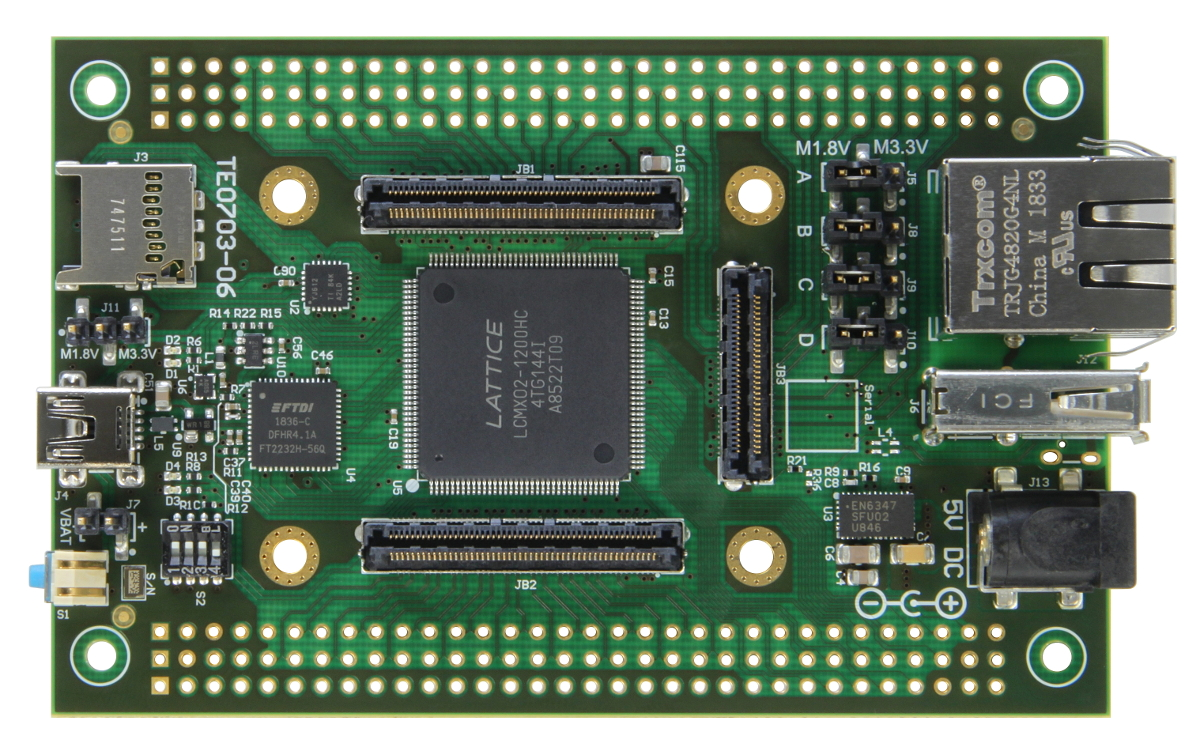
\includegraphics[scale=0.23]{imagenes/TE0703-06_1.jpg}
	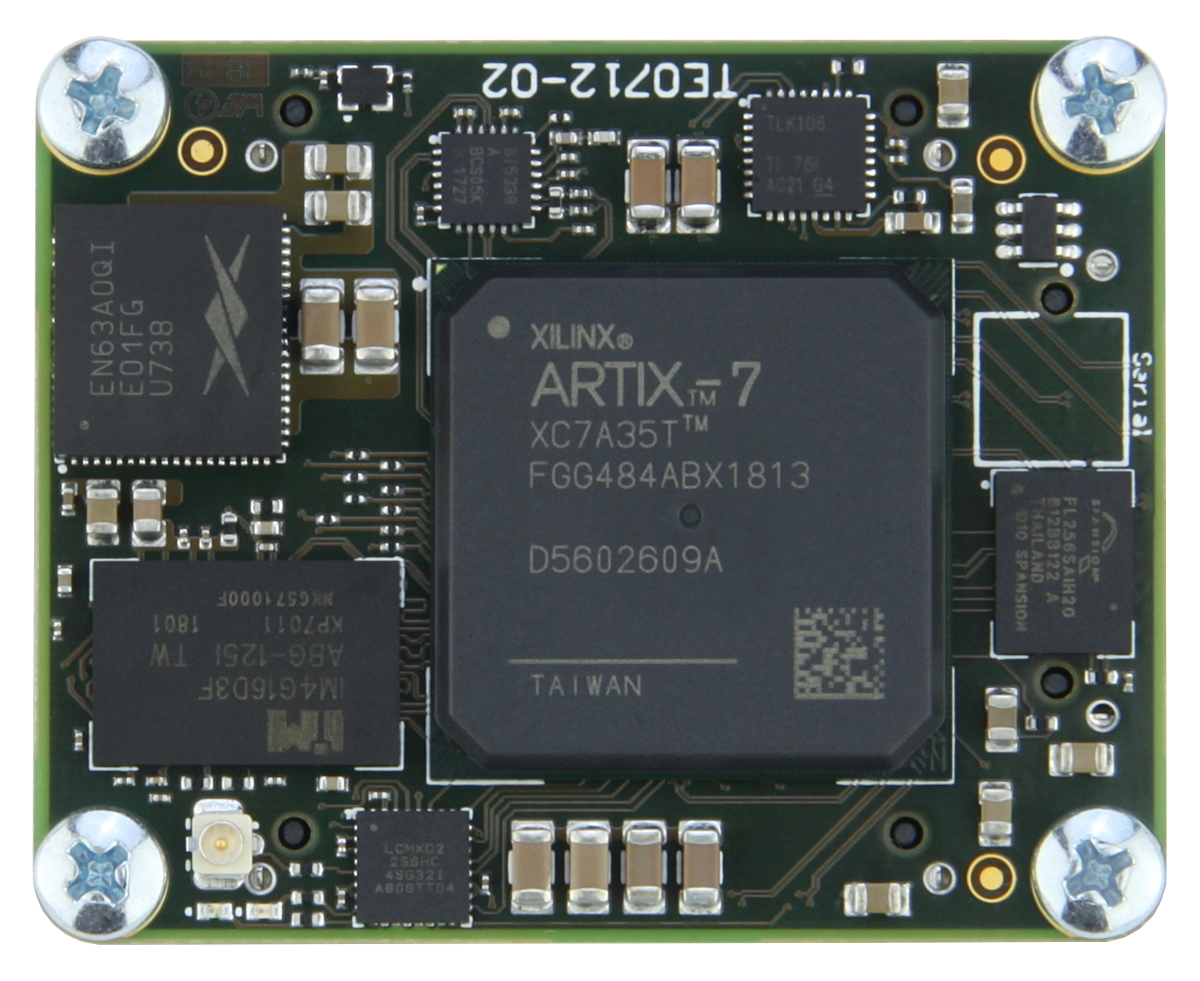
\includegraphics[scale=0.13]{imagenes/TE0712-02-35-2I_1.jpg}
	\caption{Placa de desarrollo y módulo FPGA a utilizar. A la izquierda se ilustra la placa de desarrollo Trenz TR0703\cite{TrenzElectronic2019TR0703Wiki} y a su derecha se ilustra el módulo que va montado en ella: Trenz TR0712\cite{TrenzElectronic2019TR07012Wiki} que contiene una FPGA Artix 7\cite{Xilinx20107DS180}.}
	\label{fig:trenz}
\end{figure}


Para esta alternativa de solución se consideran 32 canales de entrada LVDS ya que en el futuro será necesario conectar al menos 2 detectores de 16 canales en una misma FPGA. Para este proyecto en particular se probará el sistema con un solo detector de muones, por lo que la prueba e integración de un segundo detector queda pendiente y no se implementará en esta etapa. La figura \ref{fig:ministgc} ilustra los canales que posee un solo detector de muones de $15cm^2$.

\begin{figure}[H]
	\centering
	\includegraphics[scale=0.5]{imagenes/ministgc.pdf}
	\caption{Esquema de los canales provenientes de un detector Mini sTGC. Posee 8 tiras adyacentes de 15cm de largo por 1cm de ancho para cada eje coordenado. Cada tira emitirá un pulso analógico si una partícula cargada pasa través de ella. Se emitirán también pulsos de menor amplitud para el caso en que la partícula pase por una tira adyacente del mismo eje coordenado dentro de un radio específico. Este detector se posiciona perpendicularmente respecto a la fuente de radiación y en paralelo a (por debajo o por sobre) el sistema de disparo que indicará si la partícula captada corresponde o no a un muón. }
	\label{fig:ministgc}
\end{figure}

Las señales generadas por un detector son adaptadas por una tarjeta de interfaz ASD\cite{1999ATLASICs}, ilustrada en la figura \ref{fig:asd}. Esta tarjeta es capaz de capturar 16 señales simultaneas, por lo que es hardware suficiente para captar las señales de ambos ejes de un solo detector de muones.

\begin{figure}[H]
	\centering
	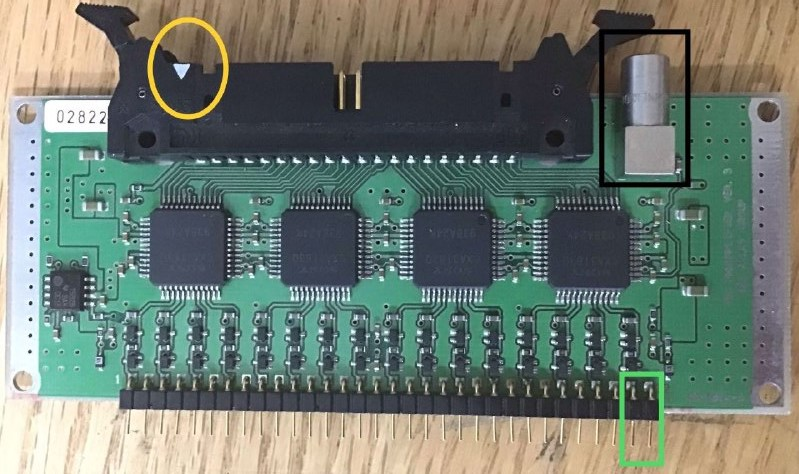
\includegraphics[scale=0.4]{imagenes/asd.jpg}
	\caption{Placa ASD\cite{1999ATLASICs} (Amplificator Shaper Discriminator), encargada de captar los 16 pulsos provenientes de un detector y entregar pulsos digitales asociados a ellos en su salida. El detector se conecta en sus entradas DIP ubicadas en su extremo inferior, mientras que las señales LVDS de salida se ubican en el conector de 40 puertos para cable plano en su extremo superior.}
	\label{fig:asd}
\end{figure}

\begin{figure}[H]
	\centering
	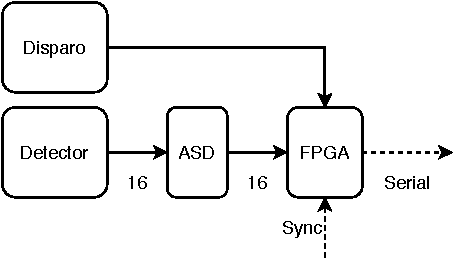
\includegraphics[scale=0.75]{imagenes/fpga1.pdf}
	\caption{Diagrama de bloques utilizando una FPGA como alternativa de solución. Se indica una salida serial para transmitir los resultados del análisis básico a algún procesador o memoria de alguna etapa posterior. La señal de sincronización ``Sync'' tiene como objetivo sincronizar la recolección y procesamiento de eventos, para que estos sean consistentes entre detectores.}
	\label{fig:fpga1}
\end{figure}


La idea en esta alternativa de solución es guardar los pulsos provenientes de la placa ASD en memoria temporal hasta la llegada de una señal de disparo. Un módulo que maneja la memoria será el encargado de tomar los pulsos correspondientes al disparo recibido y liberar la memoria de aquellos datos ya leídos u obsoletos, entregando la información útil a una siguiente etapa. Los pulsos aceptados serán entonces relacionados como parte de un mismo eventos y se estimará la duración de estos, generando y guardando así un arreglo de datos con identificador de pulso y duración. La última etapa se encargará de efectuar una operación capaz de determinar la posición del evento a partir de las duraciones medidas y los pulsos detectados, comunicando así un arreglo básico y preprocesado que incluya posición espacial y magnitud aproximada.


\begin{figure}[H]
	\centering
	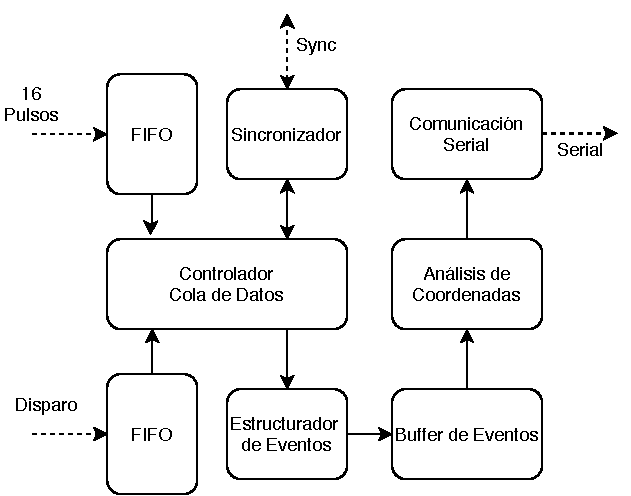
\includegraphics[scale=0.75]{imagenes/fpga2.pdf}
	\caption{Representación de la lógica interna de la FPGA. Se incluye una cola de datos para las señales de disparo, para los pulsos digitales provenientes de la ASD y una memoria de almacenamiento temporal para los eventos ya estructurados. Los bloques controlador, estructurador y análisis cumplen las funciones de aceptar o descartar pulsos, cuantificar anchos de pulso a  los canales asociados y determinar coordenada del cruce de un muón respectivamente.}
	\label{fig:fpga2}
\end{figure}

Se espera que para lograr el escalamiento se incluya una señal para mantener la lectura de eventos sincronizada entre distintas FPGA. Además, se deberá incluir un modulo de comunicación para entregar la información captada a una etapa posterior con un análisis más detallado, encargado de reunir todos los eventos de diferentes FPGAs.


%\newpage
%\section{Conclusión}
%\par Luego de presentar y evaluar diferentes alternativas de solución, el análisis indica que la mejor solución corresponde a implementar el sistema en una FPGA, obteniendo un resultado de 8.4 puntos según los criterios de selección. Esta alternativa fue precisamente la que se ha considerado desde un principio y coincide con ser la tecnología más utilizada dentro del desarrollo de sistemas de adquisición para física de partículas\cite{Basiladze2017Methods1}\cite{Basiladze2017Methods2}.
%\par Esta alternativa fue seleccionada por sobre las demás debido a su destacado desempeño, ya que cuenta con mayor frecuencia de reloj disponible, gran cantidad de recursos y suficientes puertos LVDS. Este último requerimiento es necesario para recibir los pulsos digitales capturados por la interfaz ASD provenientes del detector, los cuales se emiten bajo el estándar LVDS para transmisión de señales diferenciales.
%\par Destaca también esta alternativa al ser una plataforma flexible, en sentido de brindar las posibilidades de adaptar el diseño propuesto sin tener que adquirir nuevo equipamiento. Esta versatilidad es intrínseca de las FPGAs, las cuales se caracterizan por permitir un gran control en el diseño del hardware a bajo nivel.
%\par Luego de este trabajo de selección y detalle de la solución, ya se encuentran definidos los objetivos principales del proyecto y los esquemas generales del diseño a implementar para cumplir con ellos. Con la información presentada en la sección \ref{alternativa} es posible comenzar las etapas de planificación y posterior ejecución del proyecto, para desarrollar así un sistema de adquisición de datos para detectores de muones escalable basado en FPGA.





\newpage
\thispagestyle{empty}
\cleardoublepage

\chapter{Detección}
\label{cap:stgc}

La detección de muones en este proyecto es realizada mediante un detector de partículas inspirado en los detectores sTGC del experimento ATLAS, como se mencionó en la Sección \ref{par:smallwheel}. Los detectores originales se ubican en la llamada Small Wheel de ATLAS, formando parte del Espectrómetro de Muones, el cual se encarga de determinar el momento y la trayectoria de los muones emitidos por las colisiones. Para el proyecto sTGC minería, CCTVal construyó un prototipo de detector sTGC a menor escala utilizando la misma tecnología de fabricación presente en los detectores originales. En esta sección se describe la estructura de un sTGC original y la del prototipo en cuestión, incluyendo información sobre el funcionamiento y operación del prototipo de detector sTGC fabricado en CCTVal.

\begin{figure}[h]
	\centering
	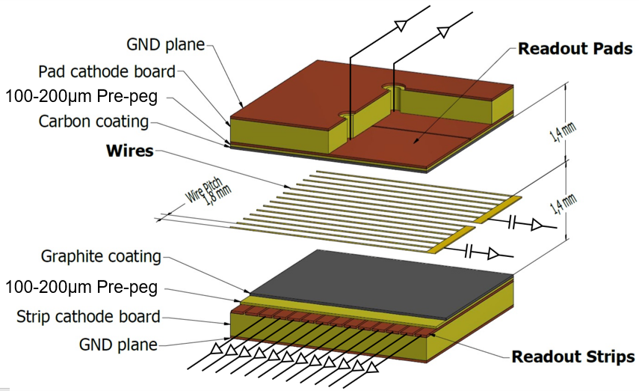
\includegraphics[scale=0.7]{tgc-structure.png}
	\caption{Estructura interna de un detector sTGC\cite{Chapman2014ATLASUpgrade}.}
	\label{img:stgc-structure}
\end{figure}

\subsection{Estructura general} 
	Un sTGC está compuesto por dos planos de grafito (cátodos), con múltiples cables en medio (ánodos)\cite{Formenti2018CERNReport}, tal como se observa en la Figura \ref{img:stgc-structure}. Recubriendo el exterior de ambos cátodos se ubican capas aislantes que separan los cátodos de las zonas conductoras, llamadas ``\textit{pads}'' en la cara superior y ``\textit{strips}'' en la cara inferior del detector, diferenciándose en la forma y área que abarca cada uno. Los \textit{strips} corresponden a delgados rectángulos de cobre, mientras que los \textit{pads} son mantos de cobre más anchos, equivalentes al área de varios \textit{strips}. Los cables al interior del detector se encuentran orientados perpendicularmente respecto a los \textit{strips} y en paralelo a los \textit{pads}.
	
	Al interior del detector, entre los planos de grafito, se infiltra un gas compuesto por dióxido de carbono y n-pentano\cite{Formenti2018CERNReport}. Mediante la aplicación de alto voltaje se genera un campo eléctrico entre ánodos y cátodos. Se utilizan 3000 V$_{DC}$ entre cátodos y ánodos para generar el campo eléctrico, limitando la corriente a 50uA. El gas en el interior puede ser dióxido de carbono puro, pero esto genera mayor probabilidad de generar descargas no asociadas a muones. La Figura \ref{img:stgc-field} representa un corte transversal de un detector y sus líneas de campo eléctrico desde ánodo (cables) hasta cátodos (lámina de grafito superior e inferior). 
	
	El paso de muones a través del detector genera la ionización del gas y la liberación de electrones, los cuales son captados por los cables del detector gracias al campo eléctrico. El flujo de electrones en el gas ionizado genera pulsos de corriente en los cables, produciendo diferencia de potencial en los cátodos. Esta diferencia de potencial interactúa con los \textit{pads} y \textit{strips} en el exterior del detector, generando pulsos de voltaje en estas zonas conductoras, pero con polaridad inversa respecto a la corriente presente en los cables. En la Figura \ref{fig:sistema-completo}, el pulso de voltaje correspondiente a la señal de salida de un canal de detección está representado por el pulso verde dibujado en la zona central de la imagen.
	
	La amplitud de los pulsos generados en el detector será mayor en torno al vértice de interacción y menor en zonas lejos de él. Esto permite relacionar la posición y energía de la partícula con las amplitudes de los pulsos en cada \textit{strip} o cable medido.
	
	\begin{figure}[h]
		\centering
		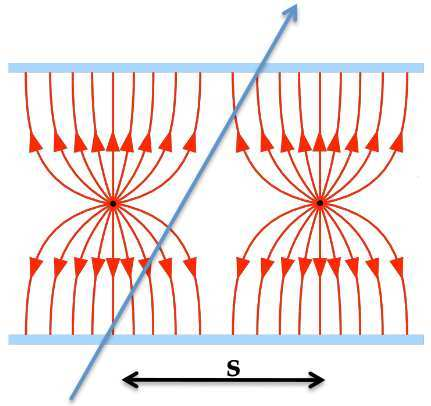
\includegraphics[scale=0.3]{stgc-transversal.png}
		\caption{Lineas de campo eléctrico observadas en un corte transversal de los cables y cátodos del detector. Los cátodos se ilustran en celeste, los cables se representan como puntos negros, y las lineas de campo corresponden a las flechas de color rojo\cite{DeSmet2011StudyLab}.}
		\label{img:stgc-field}
	\end{figure}

\subsection{Detector sTGC utilizado}
	En ATLAS, los vértices de interacción se determinan leyendo las señales provenientes de \textit{strips} y cables al mismo tiempo. Debido a que los \textit{strips} son perpendiculares a los cables, su lectura forma un cuadrante imaginario de dos ejes coordenados (\textit{strips} vs. cables), similar al presentado en la Figura \ref{img:cuadrantes-ministgc}. Por ejemplo, si un muon interactúa con un cable y un \textit{strip} al mismo tiempo, significa que el vértice de interacción se ubica en las cercanías de la intersección \textit{strip}/cable. Sin embargo, para el trabajo considerado en esta memoria de titulación se leerán solo las señales provenientes de \textit{strips}, por los que se estará midiendo un solo eje de posición y será necesario agregar un segundo eje coordenado para poder determinar los vértices de interacción. La ventaja de leer señales desde \textit{strips} es que las señales medibles en ellos son de fácil acceso, debido a que los \textit{strips} son superficies conductoras expuestas al exterior y permiten incorporar conectores sobre ellos sin mayor dificultad.
	
	Para agregar un eje coordenado adicional al detector, se reemplazan los \textit{pads} de la cara superior por \textit{strips} perpendiculares a los del plano contrario. Así se logra tener información bidimensional del paso de una partícula leyendo solo las señales provenientes de \textit{strips} perpendiculares entre sí. La Figura \ref{img:stgc-mini-estructura} ilustra la composición del detector capa por capa y detalla la orientación de cables y \textit{strips}.
	
	\begin{figure}[h]
		\centering
		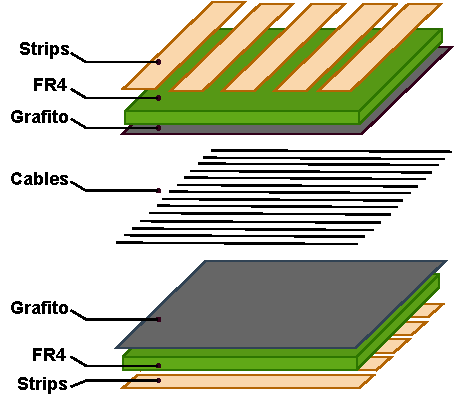
\includegraphics[scale=1]{stgc-mini-estructura}
		\caption{Estructura interna de un detector sTGC adaptado para este proyecto de titulación. El gas es contenido entre ambas capas de grafito (cátodos). Los cables internos corresponden a los ánodos.}
		\label{img:stgc-mini-estructura}
	\end{figure}

	En particular, en cada cara del detector utilizado se cuenta con 8 \textit{strips} de 15cm de largo y 1cm de ancho cada uno, sin contar los \textit{strips} en los bordes del detector debido a que el área abarcada por estos es diferente a la forma de un \textit{strip} estándar, entorpeciendo la medición y posterior reconstrucción de datos. %\sgcnote{hay strips inutiles?}\jgnote{efectivamente}.
Una fotografía de este detector se incluye en la Figura \ref{img:foto-mini-stgc}. En la parte superior de la fotografía, en recuadros verdes, se observan tubos para el flujo de gas. Por abajo, en amarillo, se indican 8 cables coaxiales conectados a los \textit{strips} de la cara superior del detector. A la izquierda están situados los otros 8 cables correspondientes a los \textit{strips} de la cara inferior, también etiquetados en amarillo. En el costado derecho, en el recuadro azul, existe una red resistiva para la lectura de cables internos del detector, los cuales no serán utilizados en este proyecto. % \sgcnote{marcar claramente estas componentes en la figura.}.
	
	\begin{figure}[h]
		\centering
		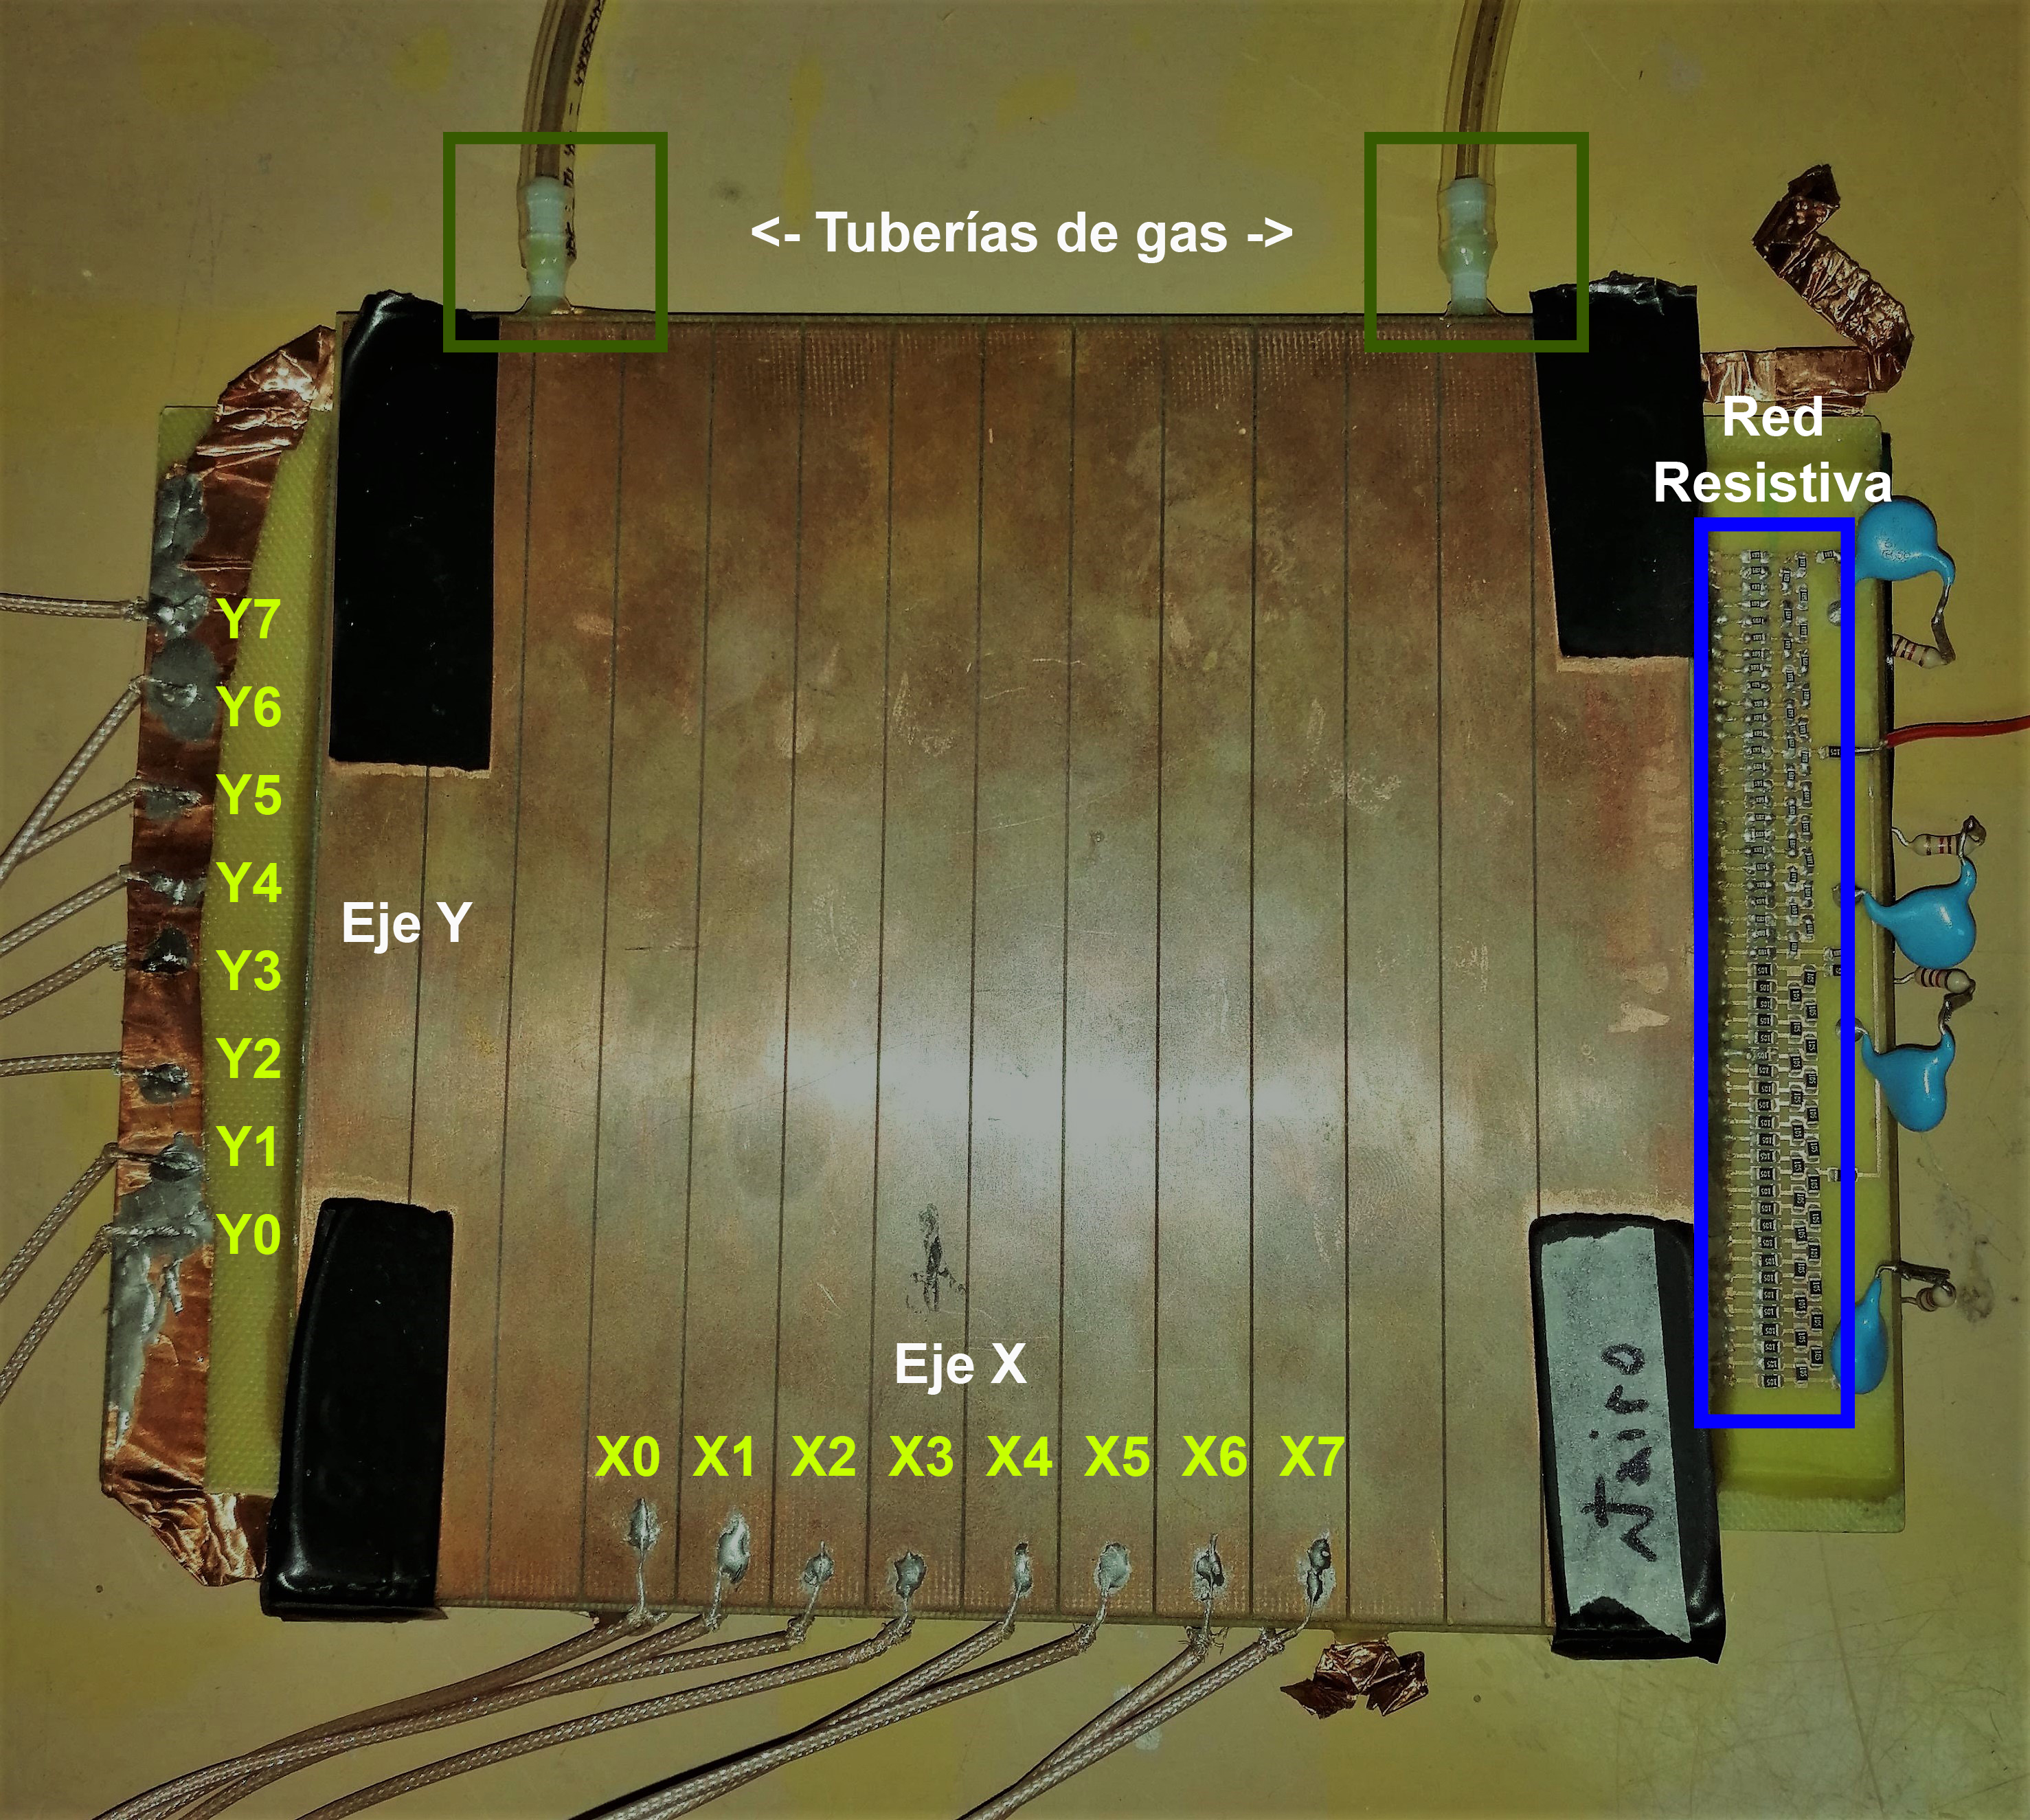
\includegraphics[scale=0.08]{mini-stgc2.jpg}
		\caption{Vista superior del detector prototipo.}
		\label{img:foto-mini-stgc}
	\end{figure}	
	
	Dado que los \textit{strips} de la cara superior del detector son perpendiculares a los de la cara inferior, es posible interpretar el detector como un cuadrante de ejes coordenados según se ilustra en la Figura \ref{img:cuadrantes-ministgc}. En esta figura, cada cuadro representa un área de detección de 1cm$^2$, la cual corresponde a la precisión para la determinación de los vértices de interacción. Como el detector posee 8 \textit{strips} por cara, se tiene un total de 16 canales de detección, los que en su conjunto forman 64 zonas de detección de 1cm$^2$. Los \textit{strips} de la cara superior se nombrarán como el eje X, mientras que los \textit{strips} correspondientes a la cara inferior del detector serán asociados al eje Y, siendo el cuadro (0,0) aquel que se ubica en la zona de detección inferior izquierda.
	
	\begin{figure}[h]
		\centering
		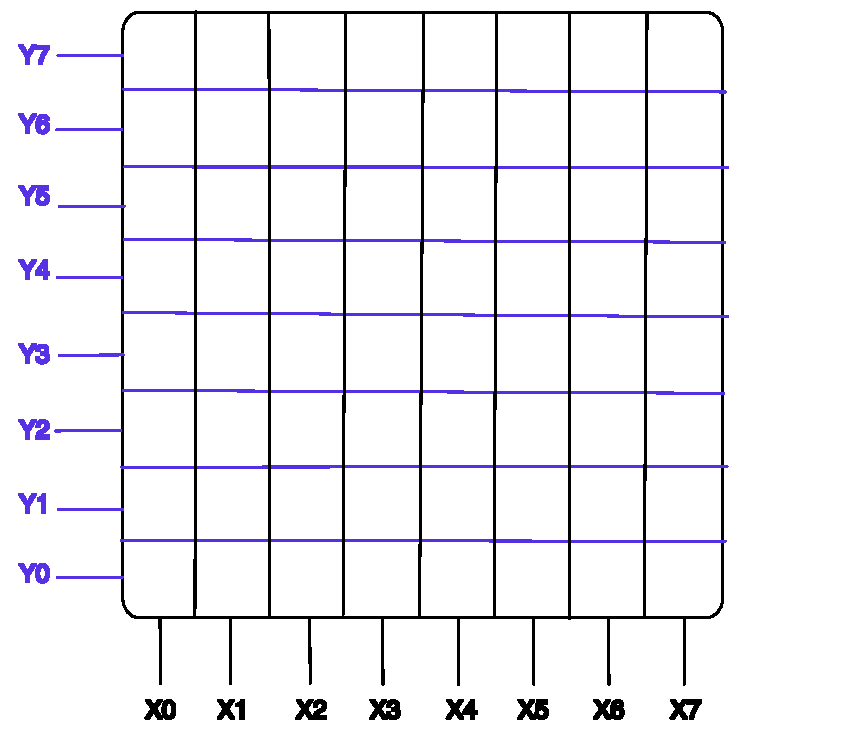
\includegraphics[scale=0.55]{cuadrantes-ministgc.pdf}
		\caption{Vista superior del detector, en donde se indican las etiquetas asociadas a cada canal en función del eje al que pertenece. Cada cuadro representa un área de detección de 1cm$^2$.}
		\label{img:cuadrantes-ministgc}
	\end{figure}

\subsection{Procedimiento de operación y pruebas}
	Antes de poner en marcha mediciones o experimentos con un nuevo detector, se deben realizar ajustes, caracterizaciones y pruebas que permitan corroborar el correcto funcionamiento del dispositivo. Para esto, se recomienda llevar a cabo una secuencia de experimentos con el fin de comprobar el funcionamiento de cada canal y medir el ruido base, la frecuencia de detección y las amplitudes medias esperadas.

	\subsubsection{Dispositivos para lectura de señales}
		Para observar los pulsos captados por el detector es necesario contar con un sistema de lectura adecuado. Este dispositivo deberá poseer una  baja impedancia, menor a 100$\Omega$ para evitar atenuaciones y reflexiones, así como también deberá contar con una etapa de amplificación tal que permita medir sin problemas las señales captadas con un osciloscopio, digitalizador o un sistema para adquisición de datos. Las señales emitidas por el detector rondan el orden de los milivolts, lo cual significa que el sistema de lectura debe poseer una ganancia tal que la magnitud de la señal de salida esté dentro de la resolución de voltaje del aparato de medición.
		
		Un ejemplo de sistema de lectura es la interfaz ASD mencionada en la Sección \ref{sec:atlas}, la cual será utilizada en este proyecto de titulación. Esta interfaz está diseñada para la correcta lectura de \textit{strips} y cables provenientes de detectores TGC, contando con una amplificación inicial de 0.8V/pC de carga y con una segunda etapa capaz de amplificar 7 veces la señal entrante. Además, la primera etapa de amplificación de la interfaz ASD se encarga de darle forma al pulso captado, con el fin extender la señal en el tiempo y facilitar su muestreo.
		
		%La interfaz ASD cuenta con salidas digitales de tipo LVDS. Estas señales representan el tiempo que la señal permanece por sobre un umbral arbitrario configurado, el cual será proporcional a la amplitud y por tanto a la carga del pulso medido. Cuenta también con una única señal análoga conectada al canal 16 (\textit{Hit} 15), proveniente de la pre-amplificación. Esta es una señal de monitoreo ideal para realizar pruebas de funcionamiento.
		

	\subsubsection{Estimación de ruido base}
		Una vez escogidos los métodos de lectura y las herramientas de muestreo a utilizar, es necesario medir el ruido base del detector. Este ruido corresponde a distorsiones propias del dispositivo, como fugas de corriente, conducción indeseada y ruido electromagnético. Conocer el ruido base permite filtrar el ruido para el análisis de eventos de interés.
		
		Para realizar la medición de ruido base en este detector prototipo se debe hacer circular el dióxido de carbono (o mezcla de dióxido de carbono y N-Pentano). Antes de proceder a realizar mediciones, es necesario esperar a que el detector haya sido llenado totalmente de gas. Dada su área interior cercana a los 225cm$^2$, el detector se encontrará completamente infiltrado con gas tras 20 minutos de operación. %\sgcnote{Especificar que estos son pasos y procedimientos para el detector en particular.  Como estan, suenan muy absolutos, como que siempre se deb hacer asi y no hay otra forma.}
		
		Cuando el detector se encuentra totalmente lleno de gas, se procede a medir el ruido base en cada uno de sus canales, sin conectar el detector a su fuente de alto voltaje. Estas mediciones permiten generar histogramas de ruido, los cuales han de tener una distribución gaussiana en condiciones normales de operación\cite{Naseri2021ATLASILC}. %\sgcnote{Puedes mostrar resultados de esto?}\sjgnote{lamentablemente no tengo datos para mostrar, es parte de las pruebas de caracterizacion del detector que se deben realizar de manera presencial de un laboratorio, pero encontre una referencia del proyecto ATLAS donde se observa ruido base en un histograma junto a otros datos sin indicar su distribucion de manera explicita. Servira?}
		
		La amplitud del ruido base definirá una zona que deberá ser considerada en los análisis de eventos. Pulsos dentro de este rango de amplitudes no serán correctamente captados. Por otro lado, se espera que el ruido sea menor que la amplitud media de los eventos generados por cruce de muones en el detector.
		
		Conocer tanto la amplitud del ruido base como la de los pulsos originados por muones, permite escoger señales de disparo en la tarjeta ASD, o filtros digitales en las etapas de análisis. 
		
	\subsubsection{Observación de falsas detecciones}
		Para una fiel interpretación de la información captada por un detector, es importante conocer la distribución y frecuencia de detecciones que no correspondan a cruce de muones. La medición de estos parámetros requiere la generación del campo eléctrico dentro del detector conectando su respectiva fuente de alto voltaje.
		
		Una vez generado el campo eléctrico, es posible captar falsas detecciones o disparos aleatorios producto de la conductividad de los materiales o fugas de corriente. Estos eventos suelen tener una distribución normal y ser de amplitudes mayores a la de interés (muones). Conocer esta información permite ignorar señales sobre un umbral tal que se correspondan con amplitudes de eventos no deseados.
	
	\subsubsection{Detección de partículas}
		Para comprobar el correcto funcionamiento del detector, es de gran utilidad utilizar fuentes radioactivas para generar pulsos de prueba. Aunque una fuente radioactiva de rayos Gamma genera pulsos de mayor amplitud que eventos producidos por muones, esta permite comprobar la correcta operación de cada canal y la distribución de carga del evento en cada canal adyacente.
	
		Para el caso de detección de muones, es importante contar con un sistema de disparo para ignorar detecciones provenientes de otras partículas cargadas capaces de ionizar el gas al interior del detector. Para el caso de sTGC, se cuenta con el sistema de detectores centelladores mencionados con anterioridad e ilustrados en la Figura \ref{fig:sistema-completo}. Se recomienda posicionar uno de estos detectores sobre el detector sTGC, cubriendo un área igual a la que abarque el sTGC. De ser factible, se recomienda incluir un segundo detector centellador por debajo, para generar una señal de disparo conjunta con el centellador superior. Esto permite descartar incidencias casi horizontales de muones, pasando por un centellador pero no por el detector sTGC.
		

%\newpage
%\thispagestyle{empty}
%\cleardoublepage
%
%\chapter{Lectura}
%\label{cap:asd}
%La interfaz de lectura ASD (Amplificator-Shaper-Discriminator)\cite{1999ATLASICs} es un sistema de 16 canales utilizado para la lectura de detectores TGC en la Big Wheel del experimento ATLAS, como se mencionó en la Sección \ref{sec:atlas}. El propósito principal de esta interfaz es detectar pulsos de alta frecuencia provenientes de detectores TGC, los cuales forman parte del Level-1 Trigger en el Espectrómetro de muones. Cada canal se corresponde con un \textit{strip} o cable de un detector, por lo que al analizar las señales de salida de esta tarjeta permite determinar los vértices de interacción \sgcnote{Revisa la gramatica, en particular tildes. Ya he corregido varios directamente en el texto, pero ya parece algo sistemativo y no puedo estar corrigiendo uno por uno.} de muones con el detector.

La Figura \ref{img:asd-board} corresponde a una fotografía de esta interfaz, destacando sus conectores principales y sus canales de entrada. Los canales son llamados \textit{Hits} y se enumeran del 0 al 15. La interfaz ASD posee \sgcnote{dangling. Quien posee?  Ultimo que corrige, ya hemos discutido como 100 veces esto} un conector de 40 pines para la conexión de su fuente de voltaje, transmisión de las señales de salida  e ingreso de pulsos de prueba \sgcnote{Revisar esto, demasiados para, para, para...}. El detalle de cada pin se ilustra en la Tabla \ref{tab:asd-ports}, donde las columnas izquierdas corresponden a los terminales positivos de los pares diferenciales, mientras que las columnas derechas indican los terminales negativos.  \sgcnote{y el punto? Mejorar la resolucion de la figura. Es una tabla. Seria mejor hacerla directo en latex.  En general, se nota que aca escribiste a la rapida sin revisar, y se nota una diferencia entre este texto y el resto (como pegado con chicle.  Debes evitar que eso se refleje en el documento.}

\begin{figure}[h]
	\centering
	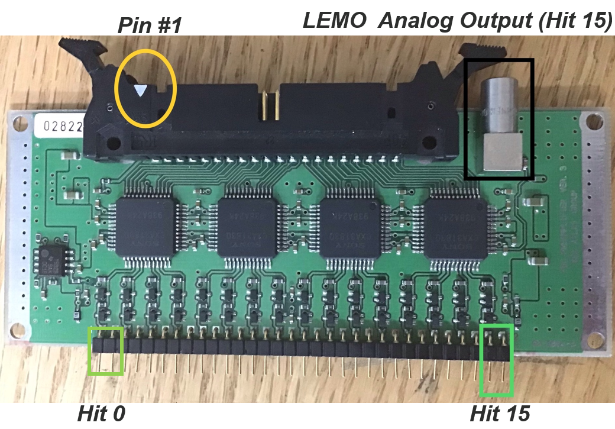
\includegraphics[scale=0.55]{asd-board.png}
	\caption{Interfaz de lectura ASD. Se destacan en la imagen sus canales (hit) del 0 al 15, su salida analógica LEMO y el primer pin en su conector de 40 posiciones.}
	\label{img:asd-board}
\end{figure}

% Please add the following required packages to your document preamble:
% \usepackage{booktabs}
\begin{table}[]
	\centering
	\begin{tabular}{@{}llll@{}}
		\toprule
		\textbf{Pin} & \textbf{Nombre} & \textbf{Nombre}                & \textbf{Pin} \\ \midrule
		1            & GND             & V$_{th}$                       & 2            \\
		3            & -3,0V           & GND                            & 4            \\
		5            & +3,0V           & +3,0V                          & 6            \\
		7            & test pulse      & $\overline{\mbox{test pulse}}$ & 8            \\
		9            & hit 0           & $\overline{\mbox{hit 0}}$      & 10           \\
		11           & hit 1           & $\overline{\mbox{hit 1}}$      & 12           \\
		13           & hit 2           & $\overline{\mbox{hit 2}}$      & 14           \\
		15           & hit 3           & $\overline{\mbox{hit 3}}$      & 16           \\
		17           & hit 4           & $\overline{\mbox{hit 4}}$      & 18           \\
		19           & hit 5           & $\overline{\mbox{hit 5}}$      & 20           \\
		21           & hit 6           & $\overline{\mbox{hit 6}}$      & 22           \\
		23           & hit 7           & $\overline{\mbox{hit 7}}$      & 24           \\
		25           & hit 8           & $\overline{\mbox{hit 8}}$      & 26           \\
		27           & hit 9           & $\overline{\mbox{hit 9}}$      & 28           \\
		29           & hit 10          & $\overline{\mbox{hit 10}}$     & 30           \\
		31           & hit 11          & $\overline{\mbox{hit 11}}$     & 32           \\
		33           & hit 12          & $\overline{\mbox{hit 12}}$     & 34           \\
		35           & hit 13          & $\overline{\mbox{hit 13}}$     & 36           \\
		37           & hit 14          & $\overline{\mbox{hit 14}}$     & 38           \\
		39           & hit 15          & $\overline{\mbox{hit 15}}$     & 40           \\ \bottomrule
	\end{tabular}
	\caption{Detalle de los puertos en el conector de 40 posiciones en la interfaz ASD.}
	\label{tab:asd-ports}
\end{table}

Como su acrónimo lo indica, la interfaz ASD (Amplificator-Shaper-Discriminator) \jgnote{Decidi introducir de nuevo esta sigla, a pesar de que ya la defini anteriormente en el primer párrafo de esta seccion y en la Seccion \ref{sec:atlas}, porque hablo especificamente de su significado} amplifica la carga eléctrica captada desde un canal de un detector, \sgcnote{por que semicolon?} modifica la forma del pulso eléctrico en cuanto a su tiempo de duración y a su amplitud de corriente con el fin de simplificar su posterior medición, y discrimina la amplitud del pulso mediante un circuito comparador. Esta comparación se realiza respecto a un nivel de voltaje ajustable para así descartar eventos de energía que estén por debajo el umbral de interés, y también para generar una señal de salida digital LVDS (Low-Voltage Differential signal)\cite{1996IEEESociety} cuya duración sea proporcional a la amplitud de pulso que ha estado por sobre el umbral de voltaje configurado. Esta técnica se conoce como TOT (Time-Over-Threshold) \sgcnote{acronimo?} y es la mísma técnica utilizada en el detector LabPet II descrito en la sección \ref{par:labpet}.  En la Figura \ref{fig:sistema-completo}, este pulso digital se representa como el pulso digital azul entre la interfaz de lectura y el sistema de adquisición de datos.
        
La interfaz ASD será utilizada conectándola a los \textit{strips} de los detectores sTGC fabricados para sTGC Minería. Dado que la interfaz posee 16 canales de entrada, es posible conectar los 16 canales de detección proveniente de un mismo detector prototipo sTGC. Así, con un solo detector y una interfaz es posible determinar vértices de interacción en un área de 225cm$^2$. Para un futuro escalamiento, utilizando dos detectores superpuestos y sus respectivas interfaces es posible determinar la trayectoria de los muones detectados. Además, analizar la duración de cada pulso emitido por las interfaces permite estimar la amplitud de la carga eléctrica depositada por el muon en el detector excitado.


\subsection{Circuito interno de Amplificación, Acondicionamiento y Discriminación}
La interfaz de lectura ASD tiene 16 canales que reciben impulsos de carga eléctrica provenientes de \textit{strips} o cables de detectores TGC, y emite señales digitales representando estos pulsos en formato LVDS según la norma IEEE LVDS Standard 1596.3-1996\cite{1996IEEESociety}.

Esta interfaz requiere una fuente de voltaje de $\pm$3V\cite{1999ATLASICs} \sgcnote{ver notacion para +-}, es capaz de recibir pulsos entre -1.2pC a +2.0pC sin saturarse y posee una frecuencia de entrada especificada \sgcnote{solo una recomendacion? No es una especificacion?} de hasta 100KHz. La interfaz cuenta con un una entrada para pulsos de pruebas y una señal analógica de monitoreo proveniente de la etapa de preamplificación del canal 15, implementada con un conector LEMO.

En la Figura \ref{img:asd-circuit} \sgcnote{mejorar la resolucion} se ilustra el circuito principal incluido en cada canal de la interfaz ASD \sgcnote{por que mayuscula?}. Cada canal tiene su propio preamplificador, un amplificador principal y un comparador\cite{1999ATLASICs}, donde la etapa de preamplificación tiene una ganancia de 0.8V/pC y el amplificador principal tiene una ganancia de 7 veces la señal entrante. La etapa de comparación compara la señal con un nivel de voltaje externo llamado \textit{V$_{th}$}. Si el pulso entrante tiene una amplitud de voltaje superior a $\frac{V_{th}}{2}$, el comparador emite una señal LVDS con una duración equivalente al tiempo durante el cual la amplitud del pulso entrante se mantuvo por sobre $\frac{V_{th}}{2}$. V$_{th}$ puede configurarse en un rango desde -0.5V a +0.5V, resultando en un umbral real de -0.25V a +0.25V en el comparador\cite{1999ATLASICs}. Así, es capaz de emitir señales digitales con duraciones entre 25ns y 45ns para pulsos de entrada con cargas entre 0.1pC y 0.5pC respectivamente.

Las señales digitales LVDS emitidas por las etapas de comparación incluidas en la interfaz ASD corresponden a las señales a ser muestreadas por el sistema de adquisición a diseñar en esta memoria de titulación. En el Capítulo \ref{cap:sdet} se define el sistema de adquisición en base a la cantidad, formato y duración de estas señales digitales.

\begin{figure}[h]
	\centering
	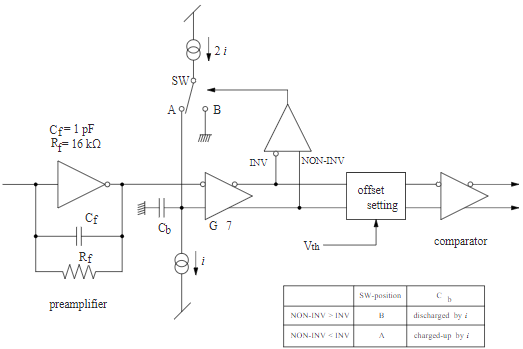
\includegraphics[scale=0.4]{asd-circuit.png}
	\caption{Diagrama de bloques del circuito principal para un canal de la interfaz ASD. Se indican la etapa de preamplificación, el amplificador principal de ganancia 7, y el comparador.}
	\label{img:asd-circuit}
\end{figure}

%\subsection{Ejemplo de operación}
%
%Por ejemplo, para un pulso proveniente de un cátodo (pulso de polaridad positiva) de 0.3pC, el voltaje esperado a la salida de la etapa de preamplificación es 240mV. La salida analógica LEMO podría reflejar un voltaje menor debido a la impedancia de la carga conectada para su lectura. Con una ganancia de 7 veces, el voltaje esperado a la salida del amplificador principal sería de 1,68V. La duración del pulso analógico sería aproximadamente 70ns, suponiendo un canto de subida con 10ns de duración y una carga proporcional a la carga de entrada. Con un voltaje V$_{th}$ de 180mV, la señal digital de salida tendría una duración de aproximadamente 50ns.
%
%La Figura \ref{img:charge-injector-output} incluye un pulso de 0.3pC de carga eléctrica, mientras que la Figura \ref{img:asd-analog-output} muestra la señal analógica en el conector LEMO. La salida LEMO presenta una amplitud de 180mV, 25\% más bajo de lo esperado, probablemente debido a la impedancia de entrada del osciloscopio utilizado para su medición

\gcnote{y esto es relevante? afecta el funcionamiento?  Falta tambien una frase de cierre que concluya y conecte con la siguientes seccion.}
\jgnote{Pensandolo bien yo diria que no es relevante este ejemplo y la diferencia entre valor esperado y medido no afecta al funcionamiento, porque se debe principalmente a que fue medido con los cables y herramientas incorrectos. Comenté esta subseccion para quitarlo del escrito.}
%
%\begin{figure}[h]
%	\centering
%	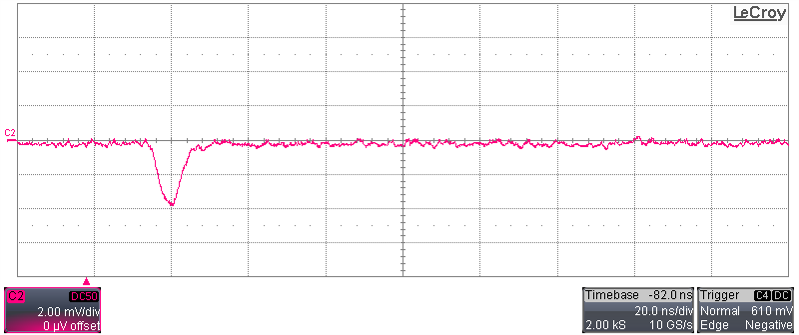
\includegraphics[scale=0.43]{charge-injector-output.png}
%	\caption{Captura de pantalla de un pulso de voltaje con carga equivalente a 0.3pC, medido en un osciloscopio.}
%	\label{img:charge-injector-output}
%\end{figure}
%
%\begin{figure}[h]
%	\centering
%	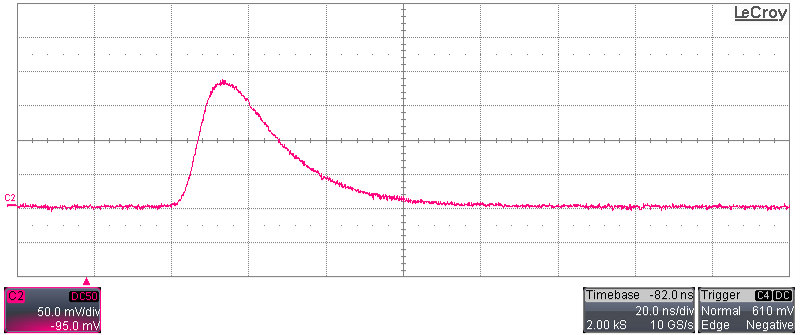
\includegraphics[scale=0.43]{asd-analog-output.png}
%	\caption{Captura de pantalla de un osciloscopio, en la cual se ilustra un pulso de voltaje proveniente de la salida analógica LEMO de la interfaz ASD luego de haber recibido un pulso de 0.3pC de carga eléctrica.}
%	\label{img:asd-analog-output}
%\end{figure}
%


%
%\newpage
%\thispagestyle{empty}
%\cleardoublepage
%
%\chapter{Muestreo}
%\label{cap:sampling}
%Detalles de la etapa de muestreo de pulsos LVDS digitales provenientes de la interfaz de lectura. Diagramas del diseño de hardware, máquinas de estado, descripción del funcionamiento, entradas y salidas, recursos utilizados.
%
%\newpage
%\thispagestyle{empty}
%\cleardoublepage
%
%\chapter{Discriminación}
%\label{cap:discriminator}
%Diseño de etapa de discriminación, para distinguir pulsos reales de falsos positivos mediante señal de trigger externo. Diagramas, maquinas de estado y recursos asociados.
%
%\newpage
%\thispagestyle{empty}
%\cleardoublepage
%
%\chapter{Estructuración}
%\label{cap:structure}
%Diseño de la etapa de estructuración, para la organización de la información capturada en estructuras de datos coherentes. La información se asocia a canales y eventos. Diagramas, máquinas de estados, recursos.
%
%\newpage
%\thispagestyle{empty}
%\cleardoublepage
%
%
%\chapter{Análisis}
%\label{cap:analysis}
%Diseño de la etapa de análisis, para asociar cuadrantes y carga eléctrica a cada evento según los datos capturados. Diagramas, máquinas de estado, variables, recursos, descripción.
%
%\newpage
%\thispagestyle{empty}
%\cleardoublepage
%
%\chapter{Sincronización}
%\label{cap:sync}
%\input{tex/Sincronizacion.tex}
%
%\newpage
%\thispagestyle{empty}
%\cleardoublepage
%
%\chapter{Comunicación}
%\label{cap:comm}
%Diseño de etapa de comunicación serial, protocolo, caracteristicas, máquina de estado, diagramas, variables, recursos, descripciones.
%
%\newpage
%\thispagestyle{empty}
%\cleardoublepage
%
%\chapter{Pruebas}
%\label{cap:test}
%Diseño de etapa de comunicación serial, protocolo, caracteristicas, máquina de estado, diagramas, variables, recursos, descripciones.
%
%\newpage
%\thispagestyle{empty}
%\cleardoublepage
%
%\chapter{Resultados}
%\label{cap:insights}
%\input{tex/Resultados.tex}
%
%\newpage
%\thispagestyle{empty}
%\cleardoublepage
%
%\chapter{Conclusiones}
%\label{cap:conclusiones}
%\section{Conclusiones}
\label{sec:conc}

Luego del trabajo realizado en esta memoria de titulación se logró cumplir con los objetivos propuestos en la Sección \ref{sec:planteamiento}. Fue posible diseñar e implementar un sistema digital capaz de cumplir con las funciones de adquirir pulsos digitales proveniente de una interfaz de lectura, discriminar la autenticidad de los eventos capturados asociados a muones y comunicar los datos adquiridos a sistemas externos, todo implementado en una tarjeta de desarrollo Trenz consistente en un SoC Zynq 7000 constituido por un procesador y lógica programable equivalente a la de una FPGA Artix 7. Las etapas de adquisición y discriminación lograron implementarse con buffers de entrada para señales LVDS y Shif-registers respectivamente, mientras que la etapa de comunicación se llevó a cabo utilizando una memoria FIFO y comunicación serial implementada en el procesador de la tarjeta Trenz.

Fue posible realizar un diseño escalable mediante el la creación de un sistema modular basado en etapas de adquisición de datos, escritura y lectura de memoria. Dado que la tarjeta Trenz cuenta con 76 pares de puertos compatibles con el estándar LVDS y con 4.9Mb de memoria distribuida en 140 bloques de 36Kb cada uno, es posible implementar con holgura dos sistemas de adquisición en una misma tarjeta, utilizando 32 puertos LVDS, 1 puerto común para señal de disparo y capacidad de almacenar hasta 2.500 eventos. Utilizando los recursos al límite, es factible implementar 4 sistemas de adquisición en una misma tarjeta Trenz, pero reduciendo la cantidad de eventos almacenables a 1.250 antes de llenar por completo la memoria FIFO. Esto no es un problema mientras los datos sean leídos de manera constante o al menos cada 1 minuto, ya que el flujo de muones en el área de detección asociada a 4 detectores corresponde a 900 eventos por minuto, llenando la memoria totalmente en cerca de minuto y medio.

La resolución espacial alcanzada por el detector es efectivamente de 1cm$^2$ mediante el cruce de canales excitados por señales de detección según el esquema de coordenadas indicado en la Figura \ref{img:cuadrantes-ministgc} de la Sección \ref{sec:stgc}. Esta resolución puede mejorar considerablemente mediante un posterior análisis de duración de pulsos detectados en canales adyacentes al vértice de interacción estimado. 

Por otro lado, la resolución temporal del sistema de adquisición diseñado fue los 2,5ns, dentro del rango de los nanosegundos, gracias a la frecuencia de reloj de 400MHz utilizada en la etapa de muestreo. Si bien esta resolución es satisfactoria, no es la máxima factible a sintetizar en la lógica programable de la tarjeta Trenz. Para lograr mayores frecuencias de reloj, es necesario cambiar el esquema de comunicación entre los módulos de muestreo y buffer de eventos, ya que pertenecen a dominios de reloj diferentes. Por ejemplo, implementar una memoria de doble puerto con operación de relojes independientes podría permitir una comunicación óptima que mejore el desempeño del sistema \gcnote{por que no se hizo esto? Ahora que lo mencionas seria como lo \emph{obvio}. Explicar/discutir.}. También es posible cambiar la manera en que se resetean algunos bloques lógicos, sobre todo aquellos encargados de retener la información de los eventos, logrando tener un \textit{fanout} mucho menor en las señales de reset utilizadas, evitando por ejemplo el restablecimiento de algunos arreglos bidimensionales y dependiendo solo de su inicialización y flujo en las máquinas de estados \gcnote{elaborar un poco mas esta discusion y las razones de por que no se hizo. Son discusiones tecnicas interesantes.}. Para alcanzar frecuencias de muestreo aún mayores, sería necesario cambiar a plataformas híbridas de adquisición de datos, como por ejemplo utilizando FPGAs en conjunto con chips DRS4\cite{RittDRS4Array} alcanzando tasas de muestreo equivalentes a utilizar un reloj de 5GHz para el caso de esta memoria. Sin embargo, frecuencias por sobre 1GHz no se justifican para la aplicación en sTGC minería, principalmente por la resolución temporal de la tarjeta ASD (no mayor a 1ns).

El haber superado satisfactoriamente prueba experimental con pulsos digitales emulados sienta precedentes satisfactorios para una posterior prueba con interfaces ASD reales y con detectores sTGC funcionales. El 100\% \gcnote{pero el 100\% de lo que hiciste es 100\% representativo de lo que pasaria en la practica? Si envie 1 dato y lo recibi, tambien podria decir que tuve un 100\% de exito.}de los datos enviados fue recibido con la resolución temporal esperada, por lo que futuras pruebas experimentales debieran tener resultados al menos similares.

Por último, el trabajo realizado, los sistemas estudiados y las herramientas utilizadas se encuentran disponibles en la enciclopedia digital de CCTVal, así como también en el repositorio de Github \cite{GonzalezMuonRepository} \sgcnote{a esto tambien deberia hacerse mencion en el capitulo 4, explicando por que es privado, y si eventualmente podria ser abierto. Aun siendo privado, seria bueno indicar si se dejho algo abierto (por ejemplo, material sobre LVDS o los wiki que hiciste)}, permitiendo la replicación, mejoramiento y continuación de este proyecto, así como también la oportunidad de adaptarlo a otros sistemas que requieran adquisición de datos en su arquitectura.


\section{Trabajo Futuro}

Para el futuro quedan pendientes muchas opciones de desarrollo interesantes. Por ejemplo, es posible fabricar una tarjeta PCB (Printed Circuit Board) que facilite la interconexión de las interfaces de lectura hacia la tarjeta Trenz. Esta PCB deberá cumplir con el estándar LVDS para señales diferenciales tomando en consideración la simetría e impedancia presente en las pistas que la compongan. Por otro lado, queda pendiente seguir mejorando el diseño digital del sistema de adquisición, poniendo al límite sus posibilidades para mejorar el desempeño en cuanto a resolución temporal. Como se menciona en la Sección \ref{sec:conc} inmediatamente anterior, es factible repensar la comunicación entre distintos dominios de reloj y optimizar la utilización de señales con alta demanda, como lo son las señales de reloj y reset. Además, es posible abarcar nuevos métodos de optimización \textit{post-placement} mediante comandos y análisis de \textit{timing}\cite{XilinxUltraFastGuide} propios de la herramienta de diseño Vivado, que podrían ayudar a alcanzar al menos los 500MHz de frecuencia de reloj.

Finalmente, queda pendiente la realización de pruebas mediante pulsos analógicos provenientes de generadores de señales y circuitos adecuados para estos fines. Además, se deberá probar el sistema con interfaces ASD reales y conectadas a sus respectivos detectores para así caracterizar el sistema completo y observar las propiedades físicas de los muones detectados. Queda pendiente también interconectar este proyecto con el sistema de disparo\cite{Oyanadel2020SistemaSTGC} fabricado por CCTVal en conjunto con el detector y la interfaz de lectura, completando así la primera etapa del proyecto sTGC Minería. Una segunda futura etapa, posterior a la adquisición de datos para detectores de muones, será la etapa de análisis de datos para reconstrucción de eventos de detección, encargada de interpretar la duración de los pulsos capturados asociados a los diferentes canales de detección. Este análisis de datos permitiría el estudio de la posición y la energía depositada por los muones en los detectores, estimar la trayectoria de los muones y determinar la densidad de la materia atravesada en su camino, logrando así generar las tomografías muónicas útiles para el estudio de terreno minero, tal como se requiere en el proyecto sTGC Minería de CCTVal.

%
%\newpage
%\thispagestyle{empty}
%\cleardoublepage


%%%------------------APÉNDICES--------------------------------

%\appendix
%\chapter{Control de versiones de proyectos Vivado con Git}
%\label{git}
%\textit{Git} es un sistema de control de versiones que permite al desarrollador crear múltiples ramas de desarrollo, sincronizar su trabajo con otros desarrolladores, revertir cambios realizados en el código y mantener una versión ordenada de un proyecto. Usar este tipo de herramientas para el desarrollo de proyectos en Vivado Desing Suite resulta ser muy útil, ya que permite trabajar de manera colaborativa y llevar registro de las versiones del hardware diseñado. En este apéndice se resumen todos los consejos y etapas para llevar a cabo el control de versiones de un proyecto Vivado. La clave del método a describir consiste subir al repositorio solo los archivos principales del proyecto, dejando fuera cualquier otro archivo proveniente de etapas de síntesis, implementación o archivos generados automáticamente por Vivado. Para llevar a cabo el control de versiones se hace uso de \textit{git} en junto con la plataforma en línea \textit{Github.com}.

Antes de comenzar, se debe contar con los siguientes requisitos:
\begin{itemize}
	\item Nociones básicas de \textit{git}.
	\item Una cuenta en \textit{Github.com}.
	\item El software de control de versiones \textit{git} instalado en el computador y habilitado para ser operado mediante un terminal de comandos.
	\item Tener instalado Vivado Design Suite (La versión utilizada en este tutorial corresponde a la versión 2019.1).
\end{itemize}

\section{Creación de un repositorio Git}

	Para comenzar, se debe iniciar sesión en \textit{Github.com} y hacer clic en el botón verde  ``New'' ubicado en la esquina superior izquierda, como se ilustra en la Figura \ref{fig:git1}.
	
	\begin{figure}[ht]
		\centering
		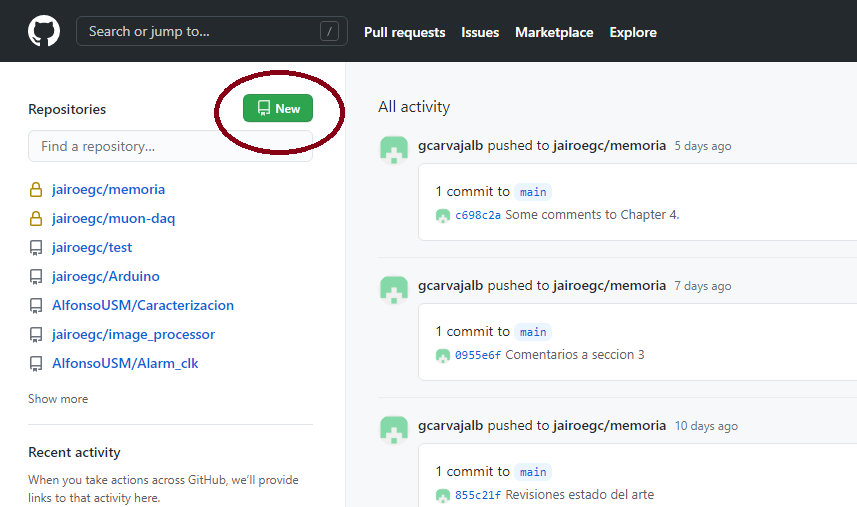
\includegraphics[scale=0.6]{git1.png}
		\caption{Botón ``New'' para la creación de un nuevo repositorio remoto en \textit{Github.com}.}
		\label{fig:git1}
	\end{figure}
	
	Se debe elegir el nombre del repositorio y configurar lo esencial. Se recomienda crear un proyecto en blanco, sin archivo \textit{readme} o \textit{.gitignore}, ya que serán subidos al repositorio de manera remota durante el primer \textit{commit}.

\section{Clonación de un repositorio Git}

	Desde la interfaz web del repositorio de Github.com debe buscarse el botón verde llamado ``Code'' (ubicado en la esquina superior derecha) y copiar en el portapapeles la \textit{URL} disponible para clonar el repositorio mediante HTTPS (Hypertext Transfer Protocol Secure), como se ilustra en la Figura \ref{fig:git2}.
	
	\begin{figure}[ht]
		\centering
		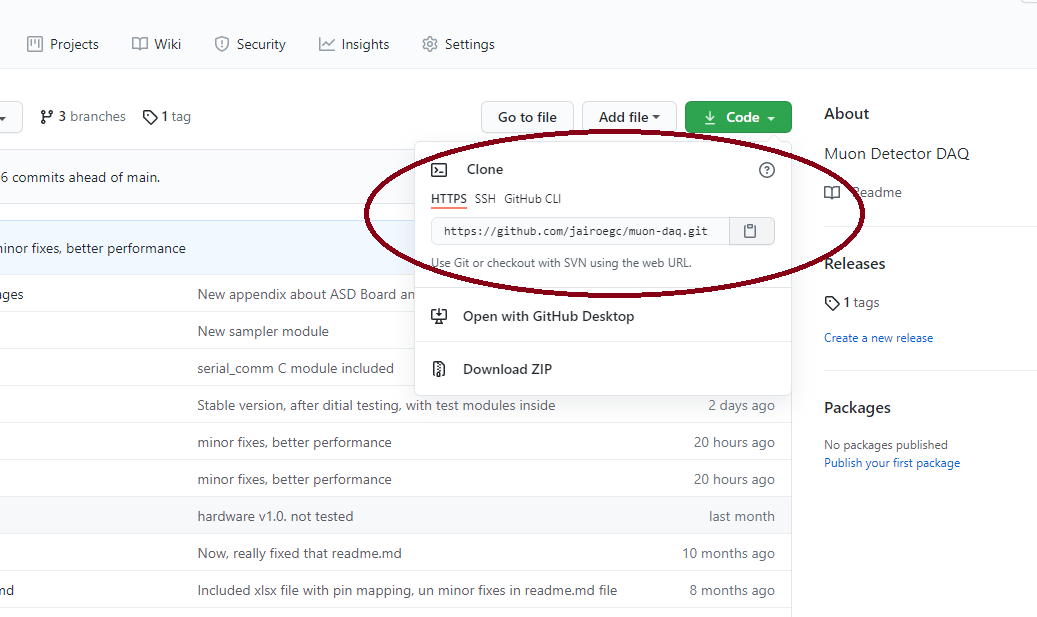
\includegraphics[scale=0.5]{git2.png}
		\caption{Botón ``Code'' para acceder al enlace de clonación del repositorio.}
		\label{fig:git2}
	\end{figure}
	
	Si aún no se tiene instalado \textit{git} en el computador, se debe proceder a su instalación vía consola o mediante descarga directa. Luego, se debe acceder o crear una carpeta para guardar el repositorio Vivado, abrir en ella una consola de comandos y escribir lo siguiente, sustituyendo \textit{your-git-url} con el enlace copiado en el portapapeles:

\begin{lstlisting}[language=bash]
$ git clone your-git-url
\end{lstlisting}


\section{Creación de los archivos y carpetas iniciales}

	Para crear los primeros archivos del repositorio se debe acceder a la carpeta escogida y crear 5 nuevas carpetas en su interior llamadas \textit{ip}, \textit{src},  \textit{sim}, \textit{xdc} y \textit{wd}.
	
	\begin{itemize}
		\item \textit{ip}: Esta carpeta incluirá los archivos asociados a IP Cores.
		\item \textit{src}: Esta carpeta es la indicada para guardar los archivos de código HDL.
		\item \textit{sim}: Carpeta para almacenar \textit{testbenchs}.
		\item \textit{xdc}: Carpeta destinada a guardar archivos XDC para \textit{constraints} y declaraciones de puertos.
		\item \textit{wd}: Esta carpeta es la indicada para guardar los archivos generados automáticamente por Vivado durante las etapas de síntesis e implementación. Esta carpeta no debe ser incluida en los \textit{commits} de \textit{git}, ya que contiene precisamente la información que no requiere seguimiento en el repositorio.	
	\end{itemize}
	
	Luego, se puede crear un archivo \textit{README.md} y uno \textit{.gitinit} en la carpeta principal. El archivo \textit{README.md} es relevante para explicar el contenido del repositorio y debe ser escrito en lenguaje \textit{Markdown}. En el archivo \textit{.gitinit} se deben incluir todos los formatos de archivo que no quieran ser subidos al repositorio, como lo son los archivos creados automáticamente por el sistema o la carpeta \textit{wd} mencionada anteriormente. Se sugiere agregar las siguientes lineas en este archivo \textit{.gitinit}:

\begin{lstlisting}[language=bash, frame=single]
wd/
.Xil/
\end{lstlisting}

\section{Preparación del proyecto Vivado}
	Antes que todo, se debe crear un proyecto Vivado y guardarlo en la carpeta \textit{wd} anteriormente creada. Si el proyecto ya existía, entonces basta con trasladar el proyecto completo y guardarlo al interior de la carpeta \textit{wd}. Luego de ello, se deben copiar o crear los archivos fuente del diseño en HDL, los archivos de simulación y los \textit{constraints} en sus respectivas carpetas.
	
	Si el diseño de hardware utiliza IP Cores, hay que asegurarse de habilitar la opción de \textit{IP Core Containers} en Vivado. Esta opción se encuentra en el menú \textit{Tools$>$ Settings$> $Project Settings$>$ IP$>$ Core Containers: Use Core Containers for IP} ilustrado en la Figura \ref{fig:viv1}, lo que facilita el control de versiones creando un solo archivo \textit{.xcix} que contiene al IP Core en su totalidad. Si Vivado pregunta por convertir el IP Core actual a un \textit{container}, dar clic en \textit{OK} y mover los \textit{containters} a la carpeta \textit{ip} correspondiente en el repositorio.
	
	\begin{figure}[ht]
		\centering
		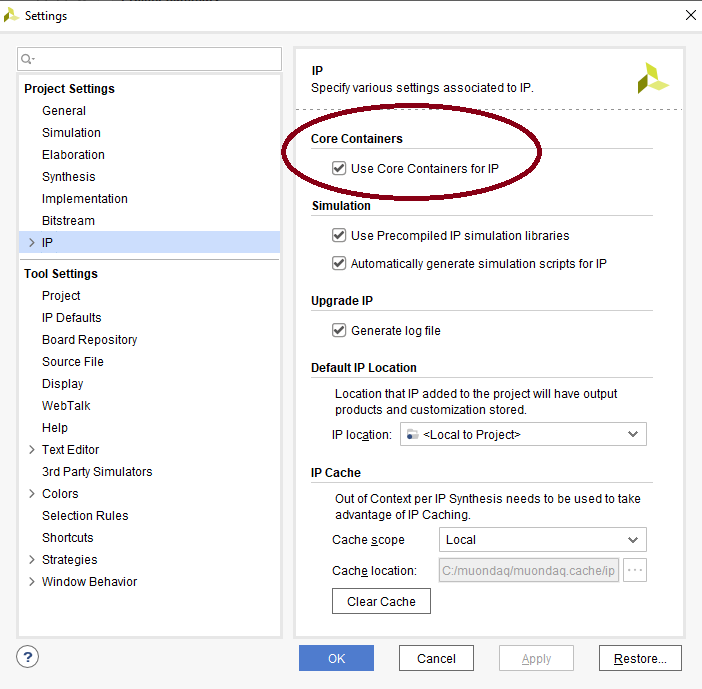
\includegraphics[scale=0.5]{viv1.png}
		\caption{Menú de configuración para la habilitación de IP Containers en Vivado.}
		\label{fig:viv1}
	\end{figure}
	
	Finalmente, se deben importar los archivos contenidos en las carpetas \textit{src, sim, xdc} e \textit{ip} al proyecto de descripción de hardware en la vista \textit{Project Manager} de Vivado.

\section{Exportar script Tcl}

	Desde la interfaz de Vivado se debe exportar el archivo \textit{Tcl} (Tool Command Language) asociado al proyecto Vivado accediendo a \textit{File$>$ Project$>$ Write Tcl} ilustrado en la Figura \ref{fig:viv2} y guardándolo con el nombre \textit{build.tcl} en la carpeta principal de repositorio, no en las subcarpetas creadas. Se debe tener encuentra que el proceso de exportación y edición del archivo Tcl debe realizarse cada vez que se crea o elimina un nuevo archivo fuente del proyecto. En caso de realizar la exportación, el script no generará el proyecto completo y habrá que importar los archivos fuente de manera manual.
	
	\begin{figure}[ht]
		\centering
		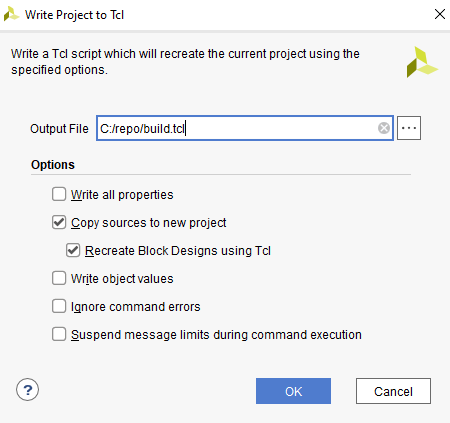
\includegraphics[scale=0.6]{viv2.png}
		\caption{Ventana de Vivado para la exportación de un script Tcl.}
		\label{fig:viv2}
	\end{figure}

\section{Editar script Tcl}
	Un paso importante en este proceso de control de versiones es la edición del archivo Tcl, para que así se generen automáticamente los archivos de Vivado en la carpeta \textit{wd}. Para lograrlo, se debe abrir el archivo \textit{build.tcl} en un editor de texto y buscar los siguientes comandos:

\begin{lstlisting}[language=bash, frame=single, basicstyle=\small]
	
# Set the reference directory for source file relative paths 
#(by default the value is script directory path)
set origin_dir "."

# Set the directory path for the original project from where
#this script was exported
set orig_proj_dir "path-to-the-actual-vivado-project"
	
# Create project
create_project ${_xil_proj_name_} ./${_xil_proj_name_} 
	-part part-of-your-fpga

\end{lstlisting}

	Una vez ubicados, se deben reemplazar por los siguientes comandos:
	
\begin{lstlisting}[language=bash, frame=single, basicstyle=\small]
	
# Set the reference directory for source file relative paths 
#(by default the value is script directory path)
set origin_dir [file dirname [info script]]

# Set the directory path for the original project from where 
#this script was exported
set orig_proj_dir "[file normalize "$origin_dir/wd/"]"

# Create project
create_project ${_xil_proj_name_} $orig_proj_dir/${_xil_proj_name_} 
	-part part-of-your-fpga

\end{lstlisting}


\section{Confirmar y subir los archivos al repositorio remoto}

	En este punto todo se encuentra listo para realizar el primer \textit{commit} en \textit{git} y comenzar el control de versiones del proyecto Vivado mediante el siguiente comando en consola:
	
\begin{lstlisting}[language=bash, frame=single]
$ git add .
$ git commit -m "First commit."
$ git push

\end{lstlisting}

	Luego de ejecutar los comandos en consola, el control de versiones se encuentra correctamente configurado y es seguro eliminar el proyecto Vivado de otras ubicaciones fuera del repositorio, ya que el proyecto puede ser reconstruido completamente al ejecutar el script \textit{ build.tcl} desde la consola Tcl de Vivado.
%
%\chapter{Conexión de señales LVDS en una FPGA Artix 7}
%\label{lvds}
%Este proyecto basa su funcionalidad en un enlace de datos físicos ente una FPGA y una interfaz de lectura ASD, en donde la interfaz emite pulsos digitales através de emisores LVDS internos y FPGA recibe los pulsos mediante un receptor interno. Este apéndice detalla cómo interconectar dispositivos que utilicen interfaces LVDS en cualquier tipo de proyecto, entendiendo los protocolos y requerimientos necesarios para lograrlo.

\section{Acerca del estándar LVDS}	
	LVDS (Low Voltage Differential Signaling) es un enlace de datos de capa física, útiles en aplicaciones que requieran principalmente conservar la integridad de los datos, mantener bajo ruido en el medio de transmisión, o cuando el emisor y receptor se encuentran demasiado lejos el uno del otro.
	
\section{Características principales}
	
	Las interfaces LVDS pueden controlar señales en el rango de los 2V a 5V, con una alta velocidad de transferencia de hasta 500Mbps en un solo par diferencial preservando la integridad de la señal a transmitir y manteniendo una buena inmunidad al ruido y a interferencia por campos electromagnéticos Se caracterizan por ser económicas, de bajo consumo de potencia, pequeñas y de una implementación simple.

	Las interfaces LVDS transfieren datos a través de una linea de par trenzado en la que los voltajes de cada alambre tienen opuesta amplitud de voltaje. Estas señales son montadas sobre un nivel de voltaje continuo típicamente de 1,2V y poseen tan solo 400mV de diferencia de voltaje ente ambos alambres. La Figura IMAGE ilustra estos niveles de voltaje.
	
	La Figura IMAGE ilustra las señales LVDS, mostrando primero una señal de una linea para luego ilustrar la señal diferencial en sí misma. V$_{idth}$ (Input Differential Threshold Voltage) corresponde al nivel de voltaje después de que el receptor capura la señal diferencial entrante.  V$_{ob}$ corresponde al alambre con potencial de voltaje positivo,  V$_{oa}$ corresponde al alambre de potencial negativo y  V$_{od}$ representa la diferencia de voltaje final ente el par de alambres.
	
	Los las interfaces diferenciales solamente emiten y reciben la diferencia entre los dos alambre que componen la linea de transmisión, eliminando el ruido de modo común en la señal de voltaje asociado a la diferencia de voltaje existente entre la tierra eléctrica , el emisor y el receptor, sumado al ruido propio infiltrado en la linea de transmisión.
	
	La implementación de una linea de datos LVDS requiere un emisor, una linea de transmisión, un resistor de 100$\Omega$ y un receptor, como se observa en la Figura IMAGE. El resistor de 100$\Omega$ se debe a la impedancia propia de la linea de transmisión (50$\Omega$) de cada alambre respecto a tierra, junto a una linea de transmisión simétrica se obtiene un medio de comunicación que mantiene la adaptación de impedancia y la integridad de la señal enviada. 


\section{Interconexión LVDS para hardware Xilinx Series 7}

	La familia de FPGAS Xilinx 7 series son capaces de operar con señales LVDS tanto en su emisión como recepción, con la opción de habilitar un resistor de 100$\Omega$ en caso de que el circuito conectado no cuente con él. Además, esta familia de FPGAS cuenta con dos tipos de estándar LVDS, el LVDS común que requiere una fuente de 1.8V y se encuentra disponible en los bancos HP (High Performance) de la FPGA, y el están LVDS\_25, el cual necesita una fuente de voltaje de 2,5V para alimentar sus bancos de puertos correspondientes unicamente a los de tipo HR (High Rank). Usar cualquiera de estos dos estándares con su correcta fuente de voltaje permita habilitar o deshabilitar el resistor interno, de lo contrario, en el caso de usar un voltaje diferente se debe mantener el resistor interno desactivado.
	
	En particular, la FPGA Artix 7 y la Zynq 7000 tienen solamente bancos HR, por lo que solo está disponible el estándar LVDS\_25, pero las tarjetas Trenz utilizadas en esta memoria de titulación solo cuentan con fuentes de 1,8V, 3,3V y 5V, lo que implica que para utilizar el resistor interno se debe utilizar una fuente de voltaje externa de 2,5V

\section{Descripción de hardware para utilización de puertos LVDS}

	Para operar correctamente utilizando puertos LVDS en la familia de FPGAs Xilinx 7 series es necesario declarar los puertos a utilizar y el voltaje asociado en el archivo de \textit{constraints} XDC. Por ejemplo para utilizar el par diferencial B16\_L22\_P (positivo) y B16\_L22\_N (negativo) ubicados respectivamente en los puertos E22 y D22 de la FPGA, se declararían las siguientes lineas:
	
	CODIGO

%set_property -dict {PACKAGE_PIN E22 IOSTANDARD LVDS_25} [get_ports B16_L22_P];
%set_property -dict {PACKAGE_PIN D22 IOSTANDARD LVDS_25} [get_ports B16_L22_N];

	Finalmente, para poder utilizar correctamente el par diferencial, es necesario utilizar un \textit{IO Buffer} instanciado en el hardware descrito. Estos buffers permiten convertir la señal diferencial a una de un solo terminal o viceversa. Por ejemplo, para usar un par diferencial según el estándar LVDS\_25 habilitando la resistencia interna del puerto, bastaria con declarar un IBUFDS (Input Buffer for Differential Singal) como se indica a continuación:
	
	CODIGO:


%// IBUFDS: Differential Input Buffer - Verilog
%// 7 Series
%// Xilinx HDL Libraries Guide, version 13.4
%IBUFDS #(
%    .DIFF_TERM("TRUE"), // Differential Termination (TRUE or FALSE)
%    .IBUF_LOW_PWR("FALSE"), // Low power="TRUE", Highest performance="FALSE"
%    .IOSTANDARD("LVDS_25") // Specify the input I/O standard (LVDS or LVDS_25)
%    ) IBUFDS_LVDS_25 (
%    .O(lvds_output), // Buffer output
%    .I(B16_L22_P), // Diff_p buffer input (connect directly to top-level port)
%    .IB(B16_L22_N) // Diff_n buffer input (connect directly to top-level port)
%);
%// End of IBUFDS_inst instantiation

Siguiendo estos pasos, el receptor LVDS queda correctamente configurado. Para utilizar el receptor basta con conectar las respectivas señales diferenciales en los puertos correspondientes declarados en el diseño y utilizar un cable de par trenzado simétrico con una impedencia de 50$\Omega$.
%
%\chapter{Ajuste de forma en pulsos electrónicos para la física}
%\label{shaping}
% 
%
%\chapter{Rayos cósmicos y partículas de alta energía}
%\label{muon}
%\input{tex/Appx_muon.tex}

%%%------------------BIBLIOGRAFÍA-----------------------------

\bibliographystyle{IEEEtran}
\bibliography{references}

\end{document}







